%% This is file `elsarticle-template-1-num.tex',
%%
%% Copyright 2009 Elsevier Ltd
%%
%% This file is part of the 'Elsarticle Bundle'.
%% ---------------------------------------------
%%
%% It may be distributed under the conditions of the LaTeX Project Public
%% License, either version 1.2 of this license or (at your option) any
%% later version.  The latest version of this license is in
%%    http://www.latex-project.org/lppl.txt
%% and version 1.2 or later is part of all distributions of LaTeX
%% version 1999/12/01 or later.
%%
%% Template article for Elsevier's document class `elsarticle'
%% with numbered style bibliographic references
%%
%% $Id: elsarticle-template-1-num.tex 149 2009-10-08 05:01:15Z rishi $
%% $URL: http://lenova.river-valley.com/svn/elsbst/trunk/elsarticle-template-1-num.tex $
%%
\documentclass[preprint,review,times,12pt]{elsarticle}

%% Use the option review to obtain double line spacing
%% \documentclass[preprint,review,12pt]{elsarticle}

%% Use the options 1p,twocolumn; 3p; 3p,twocolumn; 5p; or 5p,twocolumn
%% for a journal layout:
%% \documentclass[final,1p,times]{elsarticle}
%% \documentclass[final,1p,times,twocolumn]{elsarticle}
%% \documentclass[final,3p,times]{elsarticle}
%% \documentclass[final,3p,times,twocolumn]{elsarticle}
%% \documentclass[final,5p,times]{elsarticle}
%% \documentclass[final,5p,times,twocolumn]{elsarticle}


\usepackage[left=1in, right=1in, top=1in, bottom=1in]{geometry}
\usepackage{array}
\usepackage{multirow}
\usepackage{graphicx}
\usepackage{amssymb}
\usepackage{amsthm}
\usepackage{amsmath}
\usepackage{lineno}
\usepackage{setspace}
\usepackage{pdflscape}
\usepackage{natbib}

\journal{Ecography}
\setcitestyle{authoryear,round,semicolon,sort}
\bibliographystyle{apalike}
\begin{document}
\begin{frontmatter}

\title{Leveraging citizen science to assess richness, diversity, and abundance}

\author[DEE]{Tim M. Szewczyk}
\author[DEE]{Cleo Bertelsmeier}
\author[DEE]{Tanja Schwander}

\address[DEE]{Department of Ecology and Evolution, University of Lausanne}


\begin{abstract}
Abstract.
\end{abstract}

\begin{keyword}
Keywords
\end{keyword}

\end{frontmatter}
\linenumbers



\section{Introduction}
\label{S:1}
% Broad introduction: 
What structures ant species richness, diversity, and community structure at different spatial scales? We know that at a coarse scale, climate is generally important, with some support for phylogenetically conserved temperature preferences. At a local scale, richness typically decreases with canopy cover. In general, abundance seems to be more idiosyncratic and variable, both temporally and spatially. This is particularly true for small species. In ants, abundance can be measured as either the number of colonies in a particular area (i.e., colony density) or as the number of workers (i.e., worker density). 

Increasingly, ecologists have access to occurrence data collected in various and haphazard ways, typically in the form of online databases or citizen science projects (e.g., GBIF, BEIN, etc). These data are commonly used for species distribution models (CITE), including for individual species and hierarchical models of species communities \citep{Ovaskainen2017}, which can incorporate trait data, phylogeny, and covariation among species in addition to environmental drivers. However, they are a recent development and so far rely on a single set of occurrence data. However, use of such occurrence data for predicting richness or diversity directly has been somewhat more limited, though it is perhaps conceptually similar to extracting richness from guidebooks, which is fairly common (macroecology examples). There are several reasons for this. First, the data do not generally come from communities or assemblages, but rather an aggregation of detections from many different collectors across a variety of time spans. We like to think of diversity and richness as properties of communities, and these are decidedly not samples of communities, obscuring the ability to detect or account for interactions among species. Second, the collections for each species may have differing spatial biases, rendering any simple aggregation methods erroneous. Third, there are biases in the species that are more likely to be detected, such that any estimate of richness or diversity will necessarily be of a subset of the community biased toward larger, more active, or more interesting species.

However, that doesn't mean these data can't be useful. Instead, the geographic breadth and rather indiscriminate collection methods can capture occurrences in unexpected locations or detect species that may be missed in alternative, more structured sampling methods. Leveraging the widely available occurrence data could thus clarify patterns of species distributions and diversity, and the drivers that shape them.

Here, we combine species occurrences of ants collected in a citizen science project in western Switzerland with species abundance data from a concurrent structured sampling effort. In a hierarchical Bayesian framework, we use the citizen science data to help inform species' responses to regional variables, and the structured samples to inform responses to both regional and local variables, while accounting for bias in geographic and taxonomic sampling effort in the citizen science data. With this model, we detail the patterns of ant colony density and species diversity across the landscape while incorporating uncertainty in species compositions, and we evaluate the support for hypothesized drivers across spatial scales. We compare inferences from the combined model with those from each dataset independently, and also assess the differences in observed communities from each sampling method. 





\section{Methods}
\label{S:2}
\subsection{Study region \& sampling design}
This is a blurb about Vaud, including some about the climate, topography, as well as current and past human land use. Also a little bit about what is known about the ant fauna here, perhaps.


\begin{figure}
	\centering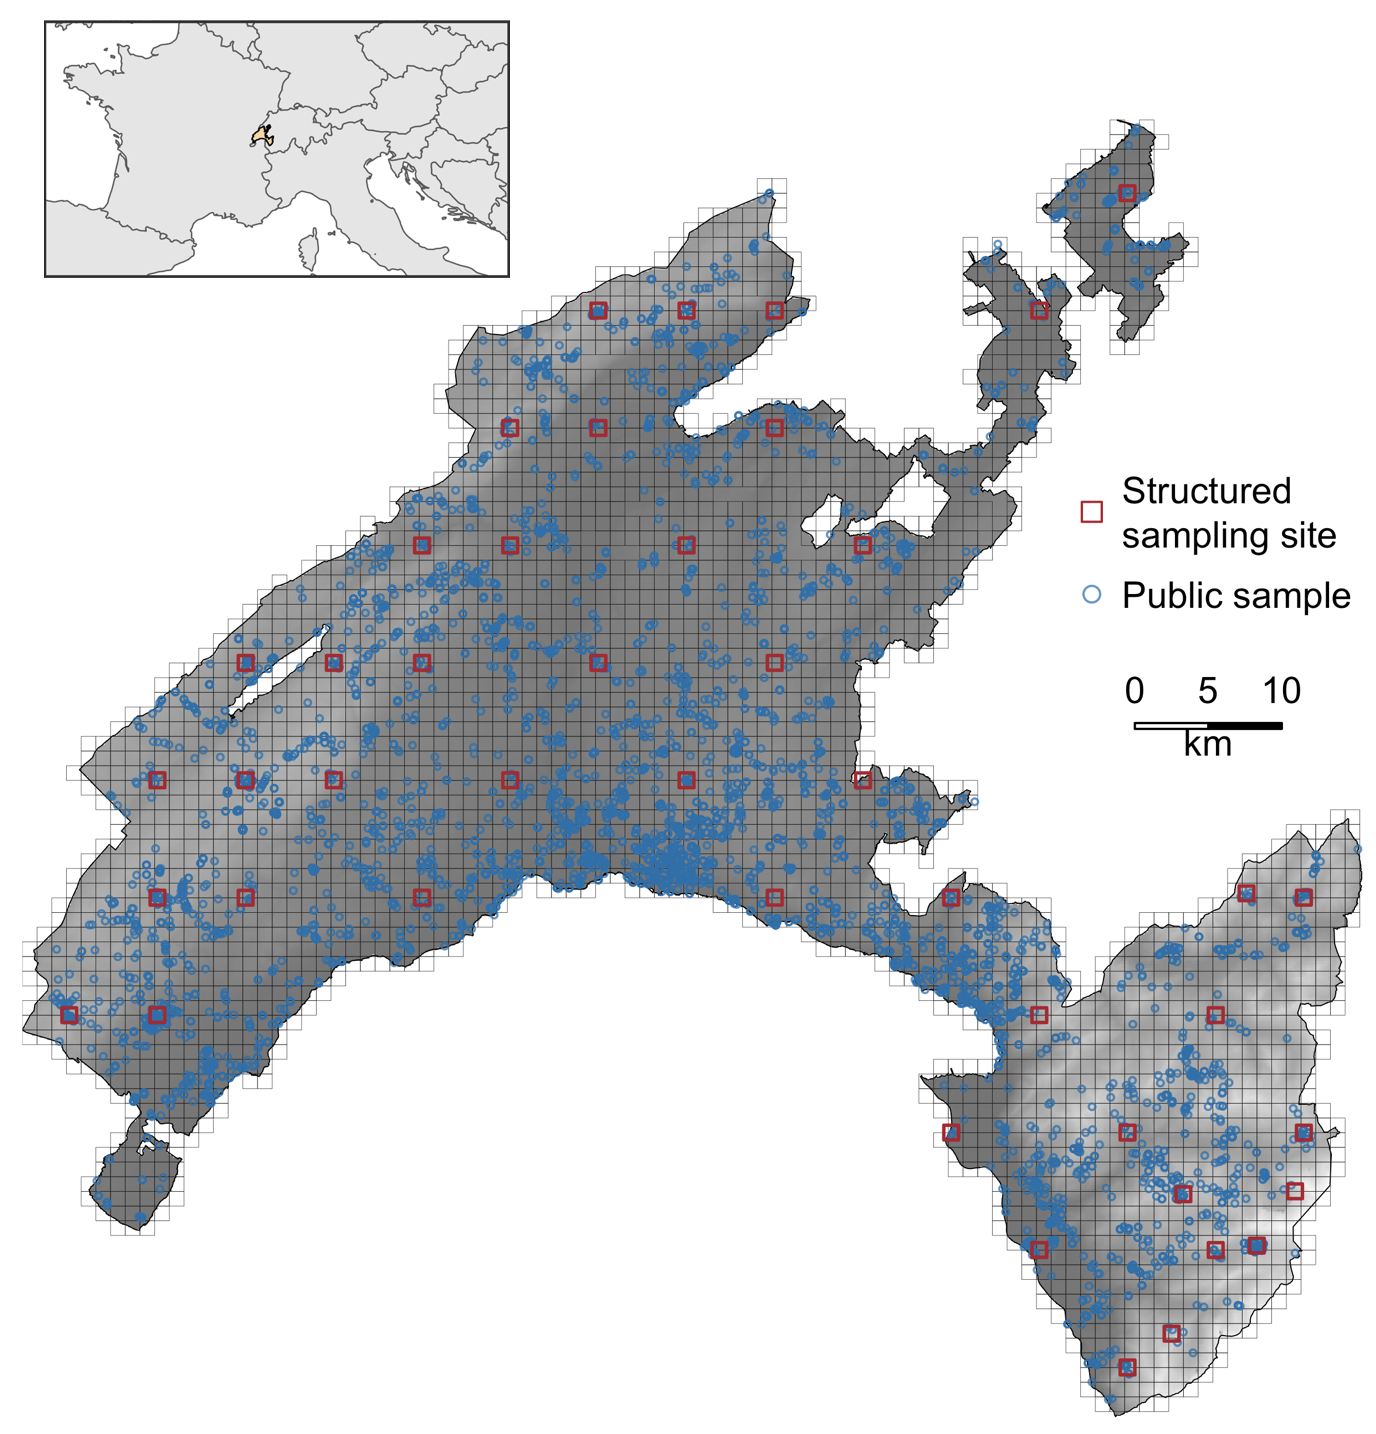
\includegraphics[width=3.5in]{ms/1_Ecography/1/figs/map_VD+inset.png}
	\caption{\label{fig:VD_map} Map of the canton of Vaud, Switzerland. Samples consisted of presence-only data (blue points) and structured abundance data collected at 1 km$^2$ long-term biodiversity monitoring sites (red squares). }
\end{figure}

% Methods for citizen science data
Ants were collected during the summer of 2019 in two simultaneous collection efforts (Fig. \ref{fig:VD_map}). First, a citizen science project (Opération Fourmis: https://wp.unil.ch/fourmisvaud/) was organized to survey the ant fauna within the canton of Vaud. Vials of ethanol were distributed to interested citizen scientists, who were asked to collect approximately 10 ant workers per colony for each vial. Participants were encouraged to explore under rocks, on bark, inside twigs, and in downed wood, and an online map was updated periodically to highlight data-sparse areas. Collectors returned the vials along with the collection date and the locality of the sample including the latitude and longitude. A total of TK samples were returned, representing collections between TK and TK. For these presence-only data, we discretized the landscape into a 1 km$^2$ grid (3,558 km$^2$) and tallied the number of counts for each species in each cell (TK cells with occurrences). 

% Methods for structured samples
Second, a structured sampling effort collected local colony abundance data, where ants were collected within 44 sites of 1 km$^2$ each, with standardized effort across sites. Thirty-nine of the sites were a part of long-term biodiversity monitoring efforts by the federal government (CITE), and as such were arranged on a regular grid with approximately 5-7 km between adjacent sites. Five additional sites are established monitoring sites by the University of Lausanne. The ants at each site were characterized by 25 plots, distributed among 15 habitat types \citep{Gago-Silva2017} in approximate proportion to the abundance of each habitat, where each habitat type present within the site was represented by at least one plot. Inaccessible areas (e.g., cliffs, water, property beyond Vaud) were excluded, resulting in several sites with areas less than 1 km$^2$, and the number of plots was reduced proportionally (TK total plots; \textbf{Appendix 1}). 

Each sampling plot consisted of a 2m radius circle, with soil temperature recorded in the center at a depth of approximately 6 cm, and vegetation characterized according to Braun-Blanquet coverage classes for grass, forb, shrub, litter, bare, and moss within the plot \citep{Douglas1978}. Six flags were evenly spaced around the circumference. Within $\sim$ 20 cm of each flag (total surface area $\sim$ 0.75 m$^2$), we searched for ant colonies within any downed wood or stumps, under large rocks, and in 2 L of soil, litter, and small rocks using 18 cm Hori Hori gardening knives. We haphazardly collected 10 workers from each colony, placing them directly into vials of ethanol. A total of TK colonies were detected across the 44 sites. Within each plot, all trees $\geq$3 cm diameter at breast height were also inspected for ant workers which were collected regardless of whether or not a colony was identifiable. Lastly, transect lines were mapped \emph{a priori}, distributed proportionally among habitat types and totalling 2 km, and surveyed at a moderate pace. Workers were collected from all permanent above-ground mounds within 2 m of the transect line. Because of the distinct sampling methods, the tree and transect collections were treated as presence-only data, and incorporated into the citizen science dataset (TK additional occurrences). 

Thus, each dataset has distinct strengths and limitations. The presence-only dataset was collected very broadly spatially, with a subset of detections resulting from free investigation of subjectively suitable habitats by skilled myrmecologists, and was therefore more likely to include rare or secretive species. However, many collections form citizen scientists occurred in or near human-dominant areas, with a likely bias toward larger, more obvious, or more anthropophilic species \citep{Ward2014, Troudet2017}. The sampling effort also varied widely across space. In contrast, the structured abundance dataset was collected with uniform sampling effort, with a sampling design aimed to produce representative samples of colony density within each site. The communities from this dataset are thus expected to be more representative of the ground-nesting ant community structure, despite detecting a smaller number of species. 

% Identification and storage
All ants were identified to species or species group based on morphology by experts (names?). Specimens are stored at the Natural History Museum of Lausanne in Lausanne, Switzerland in TK\% ethanol or mounted on pins. 


\subsection{Environmental variables}
Environmental variables were selected based on theoretical or empirical support in the literature as likely drivers of ant richness, diversity, or species distributions (CITE). At a regional (1 km$^2$) scale, we included growing degree days from ENVIREM as well as its square \citep{Title2018}, annual precipitation from CHELSA \citep{Karger2017}, net primary productivity as the average values across years 2010–2019 (MODIS: MOD17A3), the Shannon H diversity of land cover types using the proportional composition \citep{Gago-Silva2017}, the proportion of edge and forest habitats \citep{Gago-Silva2017}, the average north-facing aspect calculated as $cos(aspect*\pi/180)$ with aspect calculated from the ASTER digital elevation model \citep{Tachikawa2011}, the log-transformed total length of roads \citep{OpenStreetMap}, and the log-transformed total perimeter of buildings \citep{OpenStreetMap}. All variables were summarised as the mean or total value within each 1 km$^2$ grid cell and within each 1 km$^2$ structured site. Thus the spatial resolution was identical at the regional scale across the two datasets, though the boundaries of the structured sites do not align with the boundaries of the landscape grid.

Local variables were collected in the field at each 0.75 m$^2$ structured sampling plot as described above. We included relative soil temperature, where the recorded temperatures among plots were z-transformed within each site, as a measurement of local variation in temperature. Canopy was classified as open, closed, or mixed according to land cover type \textbf{(Appendix 1 Table X)}. Open habitats were categorized as pasture, crop, or other according to field observations. Plots within built zones or along road sides were categorized as \emph{Built} as a potential local anthropogenic effect. Finally, local productivity was quantified by using the midpoint of the range of percent cover values in each Braun-Blanquet category and summing across grass, forb, and shrub in each plot \citep{Douglas1978,Mccain2018,Szewczyk2018}.

Variable processing and summarising was performed in R 3.6.3 (CITE), with spatial computations performed using the \emph{raster} (v. 3.3.7) and \emph{sf} (v. 0.9.4) packages (CITE). All variables were z-transformed after summarising to the appropriate spatial scale to improve model behavior using the R function \emph{scale}. Additional details and references for each variable are summarised in \textbf{Appendix 1 Table X}.


\subsection{Model overview}
To leverage the strengths of each dataset, we used a community-level hierarchical inhomogenous Poisson point process model (PPM). Inhomogenous Poisson PPMs assume that the distribution of occurrences is dependent on the variation in local intensity, $\lambda(x)$, across space, $x$, which may be observed imperfectly resulting in a thinned point process \citep{Baddeley2015}. One key benefit of PPMs is that the underlying latent intensity is continuous in space, and can be integrated to arbitrary spatial resolutions \citep{Renner2015,Hefley2016,Koshkina2017a}. Following the structure of the sampling design, we modelled the expected intensity of each species at two resolutions (regional: 1 km$^2$, local: 0.75 m$^2$), representing the area of the sampling sites and the area of the sampling plots respectively. The modelled local intensities are a function of species' responses to the local and regional environment, with the structured abundance data incorporated at the local scale, and the presence-only data incorporated at the regional scale. 


\subsection{Model structure}
The hierarchical PPM unites the two datasets, \textbf{W} (presence-only citizen science collections; resolution: 1 km$^2$) and \textbf{Y} (structured local abundance collections; 0.75 m$^2$ plots within 1 km$^2$ sites). Thus, \textbf{W} informs responses to regional environmental variables, and  \textbf{Y} informs responses to both regional and local environmental variables. Similarly, \textbf{W} helps to identify overall relative abundance among species, while \textbf{Y} is a direct measurement of local abundance. We assume that local colony density for each species is a function of local and regional environmental conditions, with potential phylogenetic conservatism among species-specific responses.

The structured abundances, \textbf{Y}, are observed at the local scale. The number of observed colonies $Y_{is}$ of species $s$ at plot $i$ follows a generalized Poisson distribution with the latent colony intensity $\lambda_{is}$ and dispersion term $\theta$ to account for overdispersion \citep{Consul1992,Ntzoufras2005}. The local intensity $\lambda_{is}$ is a function of the local environment and the regional intensity of species $s$ at the encompassing 1 km$^2$ site $j$:
    \begin{equation}
        Y_{is} \sim GPoisson(\lambda_{is}, \theta) \\
        \label{eq:Y_GP}
    \end{equation}
    \begin{equation}
        log(\lambda_{is}) = a_s V_i + log(h\Lambda_{js}) \\
        \label{eq:lambda}
    \end{equation}
where \textbf{V} is a matrix of local environmental covariates, $a_s$ is a vector of species-specific responses, $h$ is a constant scaling factor representing the proportion of site $j$ sampled by plot $i$ (0.75 $m^2 /$ 1 km$^2$ = 7.5e-7), and $\Lambda_{js}$ is the regional intensity of species $s$ at site $j$. Thus, $log(h\Lambda_{js})$ functions as a site-level intercept, determining the baseline expected intensity at each plot within each site, with local intensities further dependent on the effects of the local environment \citep{Yamaura2016}.

The presence-only data, \textbf{W}, are observed at the regional scale. The number of detections of each species $s=1 \dots S$ within each 1 km$^2$ cell $k$ follow a multinomial distribution such that:
    \begin{equation}
        \{W_{ks}\}_{s=1}^{S} \sim Multinomial(\sum_{s=1}^{S} W_{ks} , \varsigma_k(\{\Lambda_{ks}D_s\}_{s=1}^{S})) \\
        \label{eq:W_Mn}
    \end{equation}
where $\{W_{ks}\}_{s=1}^{S}$ is a vector of length $S$ with the number of detections for each species within the cell, $\sum_{1}^{S} W_{ks}$ is the total number of detections within the cell, $D_s$ is the proportional detection bias for each species, which accounts for bias in the community composition based on species that are more likely to be observed, and $\varsigma_k(\cdot)$ is the softmax function which converts the weighted intensities to probabilities that sum to 1 within each cell. Therefore, for each species $s$ in cell $k$, the observed count $W_{ks}$ is expected to be higher if the species has high relative abundance ($\Lambda_{ks}$ is larger relative to other species), more samples were collected ($\sum_{s=1}^{S} W_{ks}$ is larger), or if species $s$ is likely to be over-represented in the presence-only dataset ($D_s$ is larger). 

Thus, while \textbf{W} and \textbf{Y} are each modelled with distinct sampling submodels to represent their distinct sampling methods, both $\Lambda_{js}$ and $\Lambda_{ks}$ represent the latent intensity of species $s$ at an identical 1 km$^2$ regional scale. The ecological processes driving variation in regional intensity are assumed to be the same, and the intensities are modelled together in a single regression such that:
    \begin{equation}
        log(\Lambda_{(j,k)s}) = b_s X_{(j,k)} \\
        \label{eq:LAMBDA}
    \end{equation}
where $b_s$ is a vector of species-specific slopes, and \textbf{X} is a matrix of regional environmental covariates. For each species, the average regional intensity (i.e., intercept) as well as variation across regional environments are informed by $Y_{is}$ linked through Eq. \ref{eq:Y_GP}-\ref{eq:lambda}, with the relative variation across regional environments further informed by $W_{ks}$ linked through Eq. \ref{eq:W_Mn}.  

The slopes $a_s$ and $b_s$ are species-specific responses at local and regional scales, respectively, and are distributed about genus-level means $A_g$ and $B_g$ with standard deviations $\sigma_a$ and $\sigma_b$. The genus-level means are in turn distributed about aggregate means, $\alpha$ and $\beta$ with correlation matrices $\Sigma_A$ and $\Sigma_B$, which reflect the overall responses of the ant community to environmental variables at each resolution while accounting for relatedness at the genus level \citep{Hadfield2010b,Szewczyk2018}.

Prior distributions were lightly informative to constrain the sampling algorithm to plausible ranges. Specifically, aggregate slopes $\alpha$ and $\beta$ were distributed Normal($\mu=0$, $\sigma=1$), the intensity intercept $\beta_0$ was distributed Normal($\mu=-4$, $\sigma=2$), standard deviations for species and genus slopes were distributed Normal($\mu=0$, $\sigma=2$) and constrained to be positive, the correlation matrices used a Cholesky decomposition and followed an LKJ prior as recommended for better model fitting (CITE) with $\eta=2$, and the proportional taxonomic bias term $D$ was distributed Normal($\mu=1$, $\sigma=1$) and constrained to be positive. Code for the full model is available on GitHub (https://github.com/Sz-Tim/CH\_diversity).

Finally, several quantities were calculated at the regional and local scales for each sample from the posterior. Probability of presence was calculated as $1 - e^{-\Lambda_{(j,k)s}}$ at the regional scale  \citep{Hefley2016}, and $1 - pr(0 | \lambda_{is}, \theta)$ at the local scale. Predicted richness was calculated within each plot or grid cell as the sum of the species with $\geq$ 95\% probability of presence. Shannon's H was calculated at each plot using $\lambda_{i,1-S}$ and in each cell using $\Lambda_{(j,k),1-S}$. Total predicted intensity was calculated as $\sum_{s=1}^{S}\Lambda_{(j,k)s}$ and $\sum_{s=1}^{S}\lambda_{is}$. Thus, posterior predictions of local patterns were based only on the local plots at the 44 structured sites, while those of regional patterns were based on the 44 structured sites and the entire gridded landscape for Vaud (Fig. \ref{fig:VD_map}). 


\subsection{Variable selection \& model fitting}
To evaluate the effect of including the presence-only data, \textbf{W}, we compared a version of the model with and without \textbf{W}. We refer to the model that uses both \textbf{W} and \textbf{Y} as the \emph{Joint} model, and the model using only \textbf{Y} as the \emph{Structured} model. The \emph{Structured} model therefore does not include Eq. \ref{eq:W_Mn}, but nevertheless includes species only detected in \textbf{W}. We performed variable selection separately on the two models.

Because comparing all possible models was not feasible, variable selection was performed using a 4-fold cross-validation with a step-wise forward search. The 44 sites in the structured abundance dataset \textbf{Y} were divided into 4 subsets using the \emph{caret} (v. 6.0.86) R package (CITE). The models were parameterized using 3 of the subsets and predictive ability assessed using the 4$^{th}$, with four separate model runs such that all subsets were predicted once. In each round, the log pointwise predictive density of the observed abundances given the predicted local intensities for each candidate model was calculated and compared using the \emph{loo} (v. 2.3.1) R package (CITE). Variables were added sequentially until predictive ability unambiguously declined, and the variable sets for the \emph{Joint} and \emph{Structured} models with the best out-of-sample predictive ability were considered optimal.

All Bayesian models were written in Stan (CITE) and run in \emph{CmdStan 2.23.0} (CITE). In contrast to BUGS or JAGS, which use Gibbs samplers for the Markov Chain Monte Carlo algorithm, Stan uses a Hamiltonian Monte Carlo algorithm which requires a warm-up period to tune the sampler parameters rather than a burn-in period. During variable selection, we ran 3 chains for each model with 2,500 iterations per chain, with 2,000 iterations for the warm-up period. For the optimal models, we ran 12 chains with 2,250 iterations each, with 2,000 iterations for the warm-up period. Model behavior and convergence was assessed by confirming that all $\hat{R}$ values were $\leq$ 1.1, visually inspecting a selection of trace plots, and confirming that no divergent transitions occurred during the sampling, which would indicate a poor approximation of the joint posterior distribution. Highest Posterior Density Intervals (HPDIs) were calculated for all parameters of interest using the \emph{HDInterval} (v. 0.2.2) R package (CITE).


\subsection{Community analyses}
Using the $\lambda$ posterior medians, we calculated the $\beta$-diversity among plots within each site using the \emph{betapart} (v. 1.5.1) R package (CITE). The overall $\beta$-diversity at each site was partitioned into the balanced variation and abundance-gradient components, representing changes in relative abundance among species and changes in total abundance, respectively \citep{Baselga2017}. Change across elevation was assessed using linear and quadratic regressions compared with AICc using the \emph{AICcmodavg} (v. 2.3.0) R package (CITE). A double principal coordinates analysis (DPCoA) was also performed using $\lambda$ posterior medians to assess similarity in taxonomically-weighted community structure among plots \citep{Dray2015,Pavoine2019} using the \emph{ade4} (v. 1.7.15) and \emph{vegan} (v. 2.5.6) R packages (CITE). 




\section{Results}
\label{S:3}
A total of 80 species were detected across both datasets, with TK in the presence-only dataset and TK in the structured abundance dataset. The total number of samples in each dataset, the number of grid-cells with presences in the public dataset, the range of counts across cells. The species only detected in one but not the other, and then vice versa.

% Model performance & covariates
In the 4-fold cross-validation, the model parameterized with both the presence-only and structured abundance datasets (\emph{Joint} model) consistently outperformed the model parameterized with only the structured abundance dataset (\emph{Structured} model) in predicting local abundances (Table?). Both optimal models included growing degree days at a regional scale, and local effects of canopy type, cropland, and pastureland (Fig. \ref{fig:slope_means}). The optimal \emph{Joint} model also included regional effects of annual precipitation, forest proportion, and road length, and local effects of soil temperature. For many variables, species showed a variety of responses, resulting in no clear aggregate effect as the 95\% Highest Posterior Density Intervals (HPDIs) for $\beta$ included zero. However, the aggregate effect of growing degree days was positive in the \emph{Joint} model, and the aggregate effects of squared growing degree days and cropland were negative in both models. For soil temperature, pasture, and mixed canopy, nearly all species with non-zero HPDIs showed positive responses (\textbf{Appendix 2 Figure}). The \emph{Joint} model reduced uncertainty in species' responses compared to the \emph{Structured} model across most covariates (Fig. \ref{fig:slope_means}b). This reduction occurred on average across all species, but was greater for species that did not occur in the structured abundance dataset \textbf{Y}.

\begin{figure}
\centering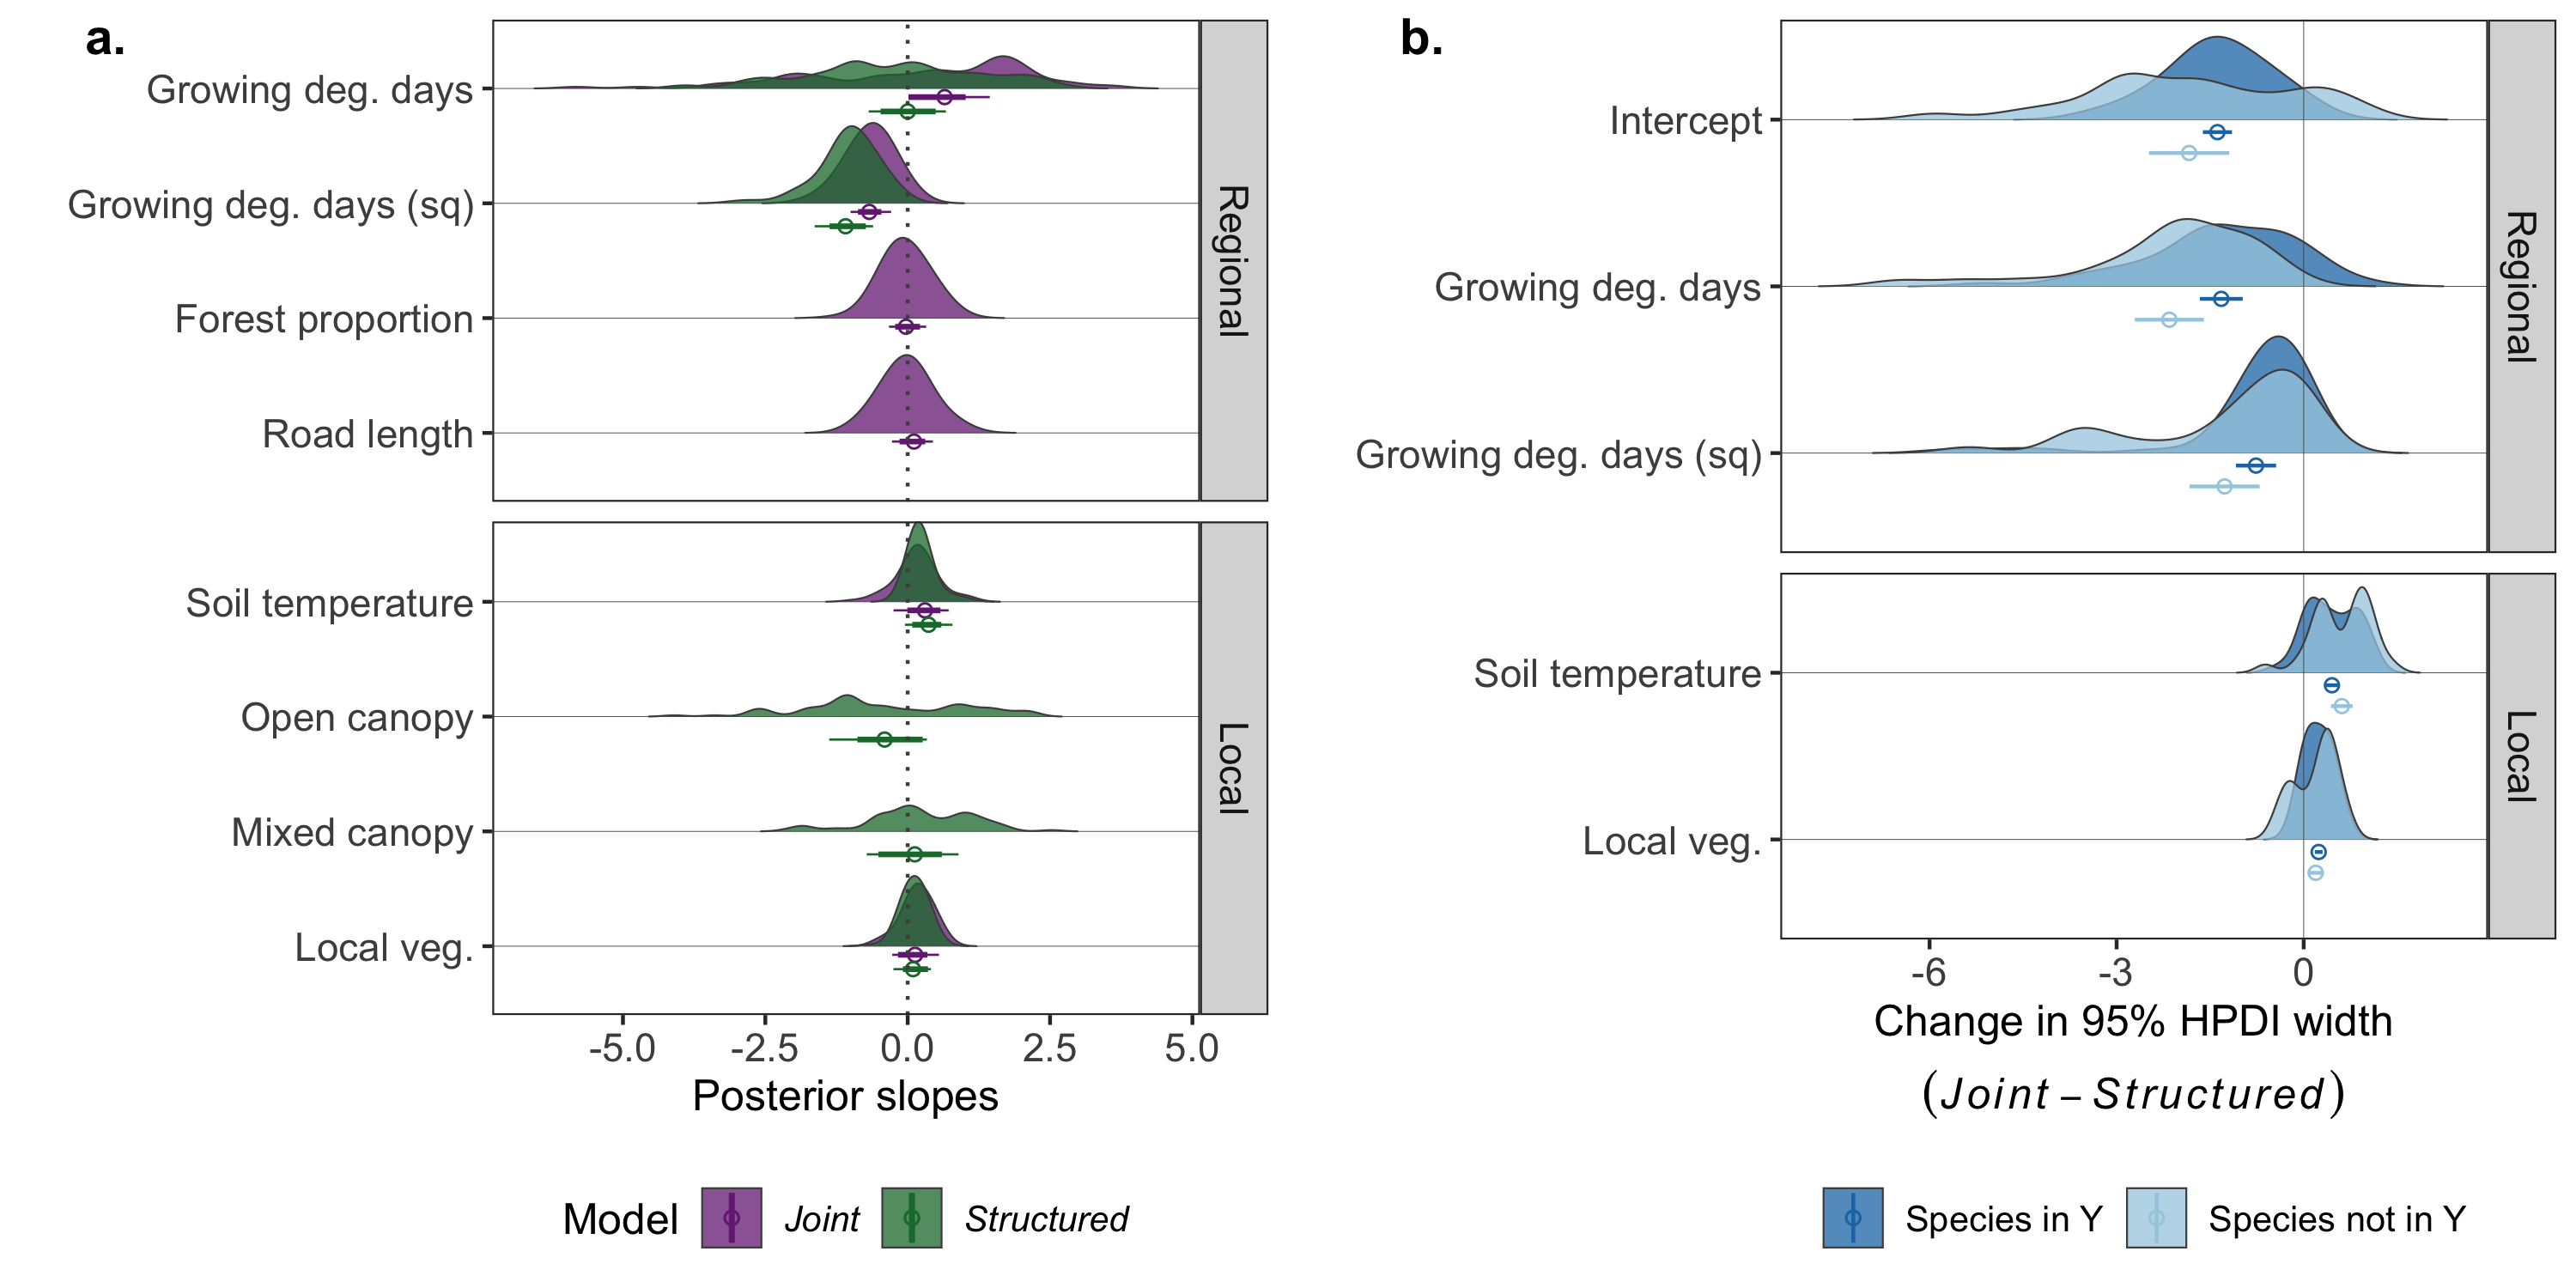
\includegraphics[width=6in]{ms/1_Ecography/1/figs/slope_means+HDI.png}
\caption{\label{fig:slope_means} Covariate effects in optimal models. (a) Density curves summarise species-level posterior means for responses to variables in the model using both datasets (\emph{Joint}: purple) and the model using only the abundance data (\emph{Structured}: green). Points and lines show posterior means and Highest Posterior Density Intervals (HPDI; thick: 80\%; thin: 95\%) for the aggregate ($\beta$) responses. (b) Change in 95\% HPDI widths in species responses between models (negative: less uncertainty in \emph{Joint} model) for species observed in the structured abundance dataset \textbf{Y} (dark blue) or only in the presence-only dataset \textbf{W} (light blue). Points and lines show mean $\pm$ standard error across species. }
\end{figure}

% Elevational patterns
Across the canton of Vaud, predicted ant richness showed a peak just below 1000m at a regional scale, with no clear trend at a local scale for the plots within the 44 structured sites (Fig. \ref{fig:el_patterns}a), regardless of whether the model was parameterized with both datasets (\emph{Joint}) or only the local structured abundance dataset (\emph{Structured}). In contrast, the \emph{Joint} model predicted higher regional Shannon diversity at lower elevations, while the \emph{Structured} model predicted a peak near 1000m (Fig. \ref{fig:el_patterns}b). Both models predicted lower local Shannon diversity at low elevations, though the \emph{Structured} model predicted a more dramatic increase from 300m–1000m. The \emph{Structured} model predicted higher regional colony intensities at lower elevations, in contrast to the more constant intensities predicted by the \emph{Joint} model (Fig. \ref{fig:el_patterns}c). Local predicted intensity was similar across models, with a slight dip near 1000m and a decline toward the highest elevations. 

\begin{figure}
	\centering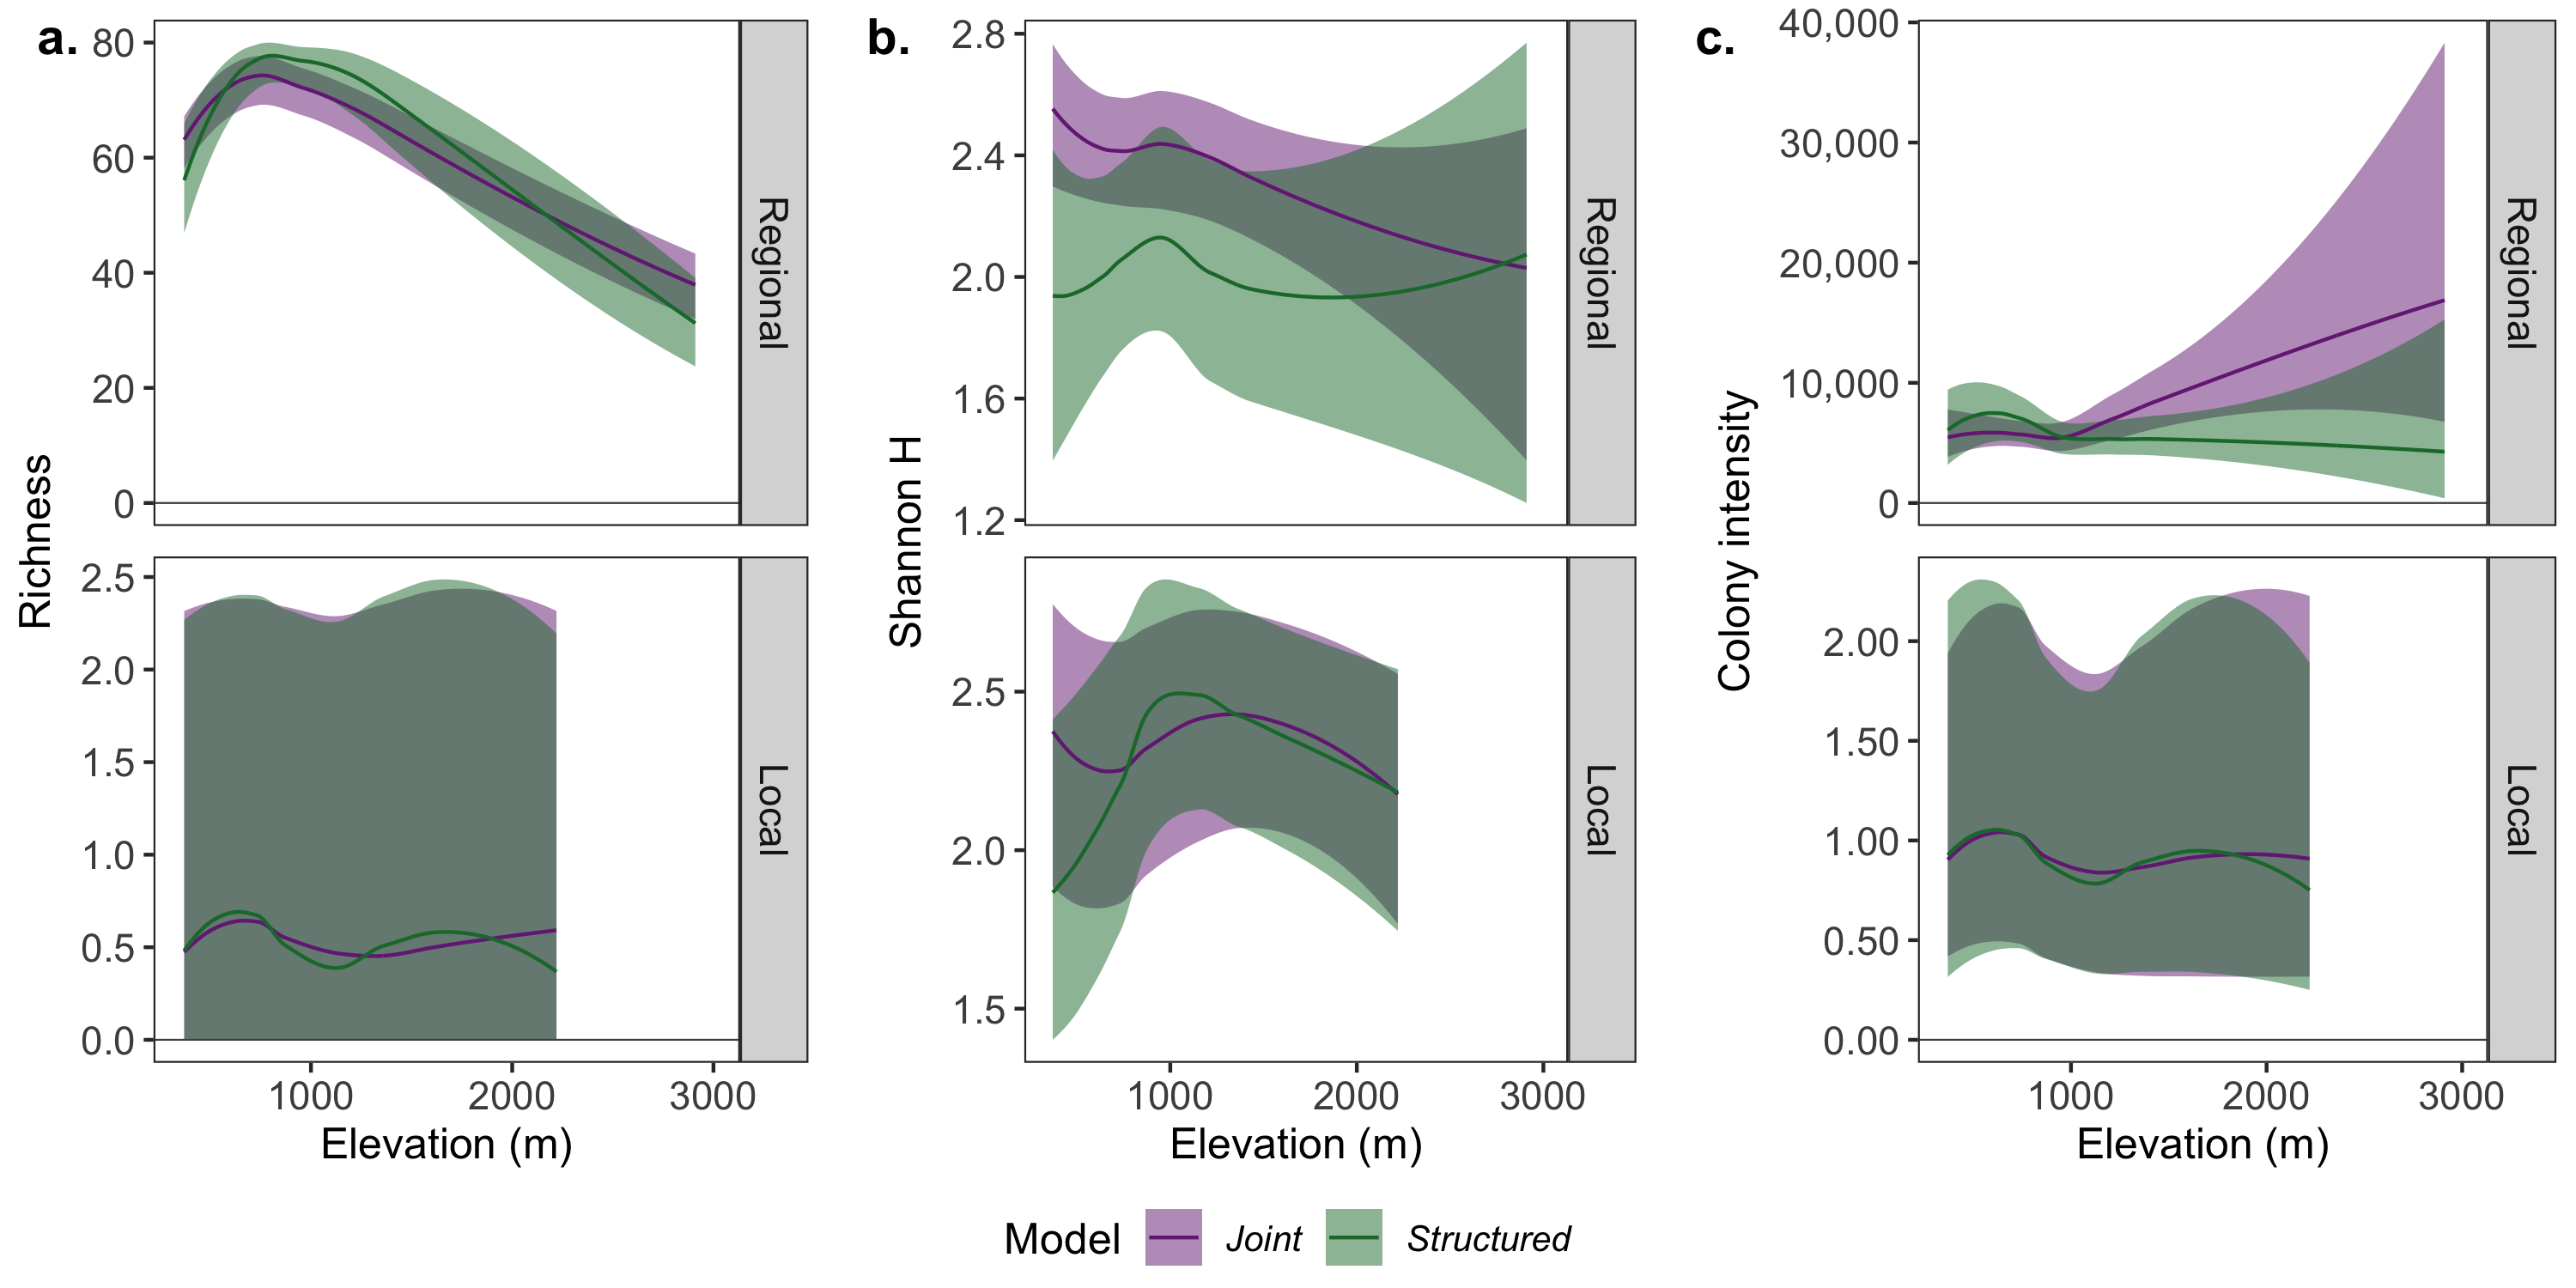
\includegraphics[width=6in]{ms/1_Ecography/1/figs/el_patterns.png}
	\caption{\label{fig:el_patterns} Elevational patterns of posterior distributions at regional and local scales for (a) species richness, (b) Shannon H diversity, and (c) total colony intensity. Lines and ribbons are loess lines using the posterior medians and 95\% Highest Posterior Density Interval, respectively, for the model parameterized with both datasets (\emph{Joint}: purple) and the model parameterized with only the structured abundance data (\emph{Structured}: green). }
\end{figure}

The local ant communities showed strong separation across elevations. Using the posterior median local communities predicted by the \emph{Joint} model, communities formed two distinct clusters representing plateau ($<$1000m) and montane ($\geq$1000m) plots (Fig. \ref{fig:dpcoa}). The DPCoA accounts for relatedness among species, with the 100m elevational bins (Fig. \ref{fig:dpcoa}a) or regions (Fig. \ref{fig:dpcoa}b) applied \emph{post-hoc}. No clear pattern is seen at elevations $<$1000m, while elevation increases down the y-axis at elevations $\geq$1000m. Plateau communities form a broader cluster, indicating greater variation among local ant communities. Montane communities form a smaller cluster, with little differentiation in the communities found in the western Jura mountains and those in the eastern Alps.

\begin{figure}
	\centering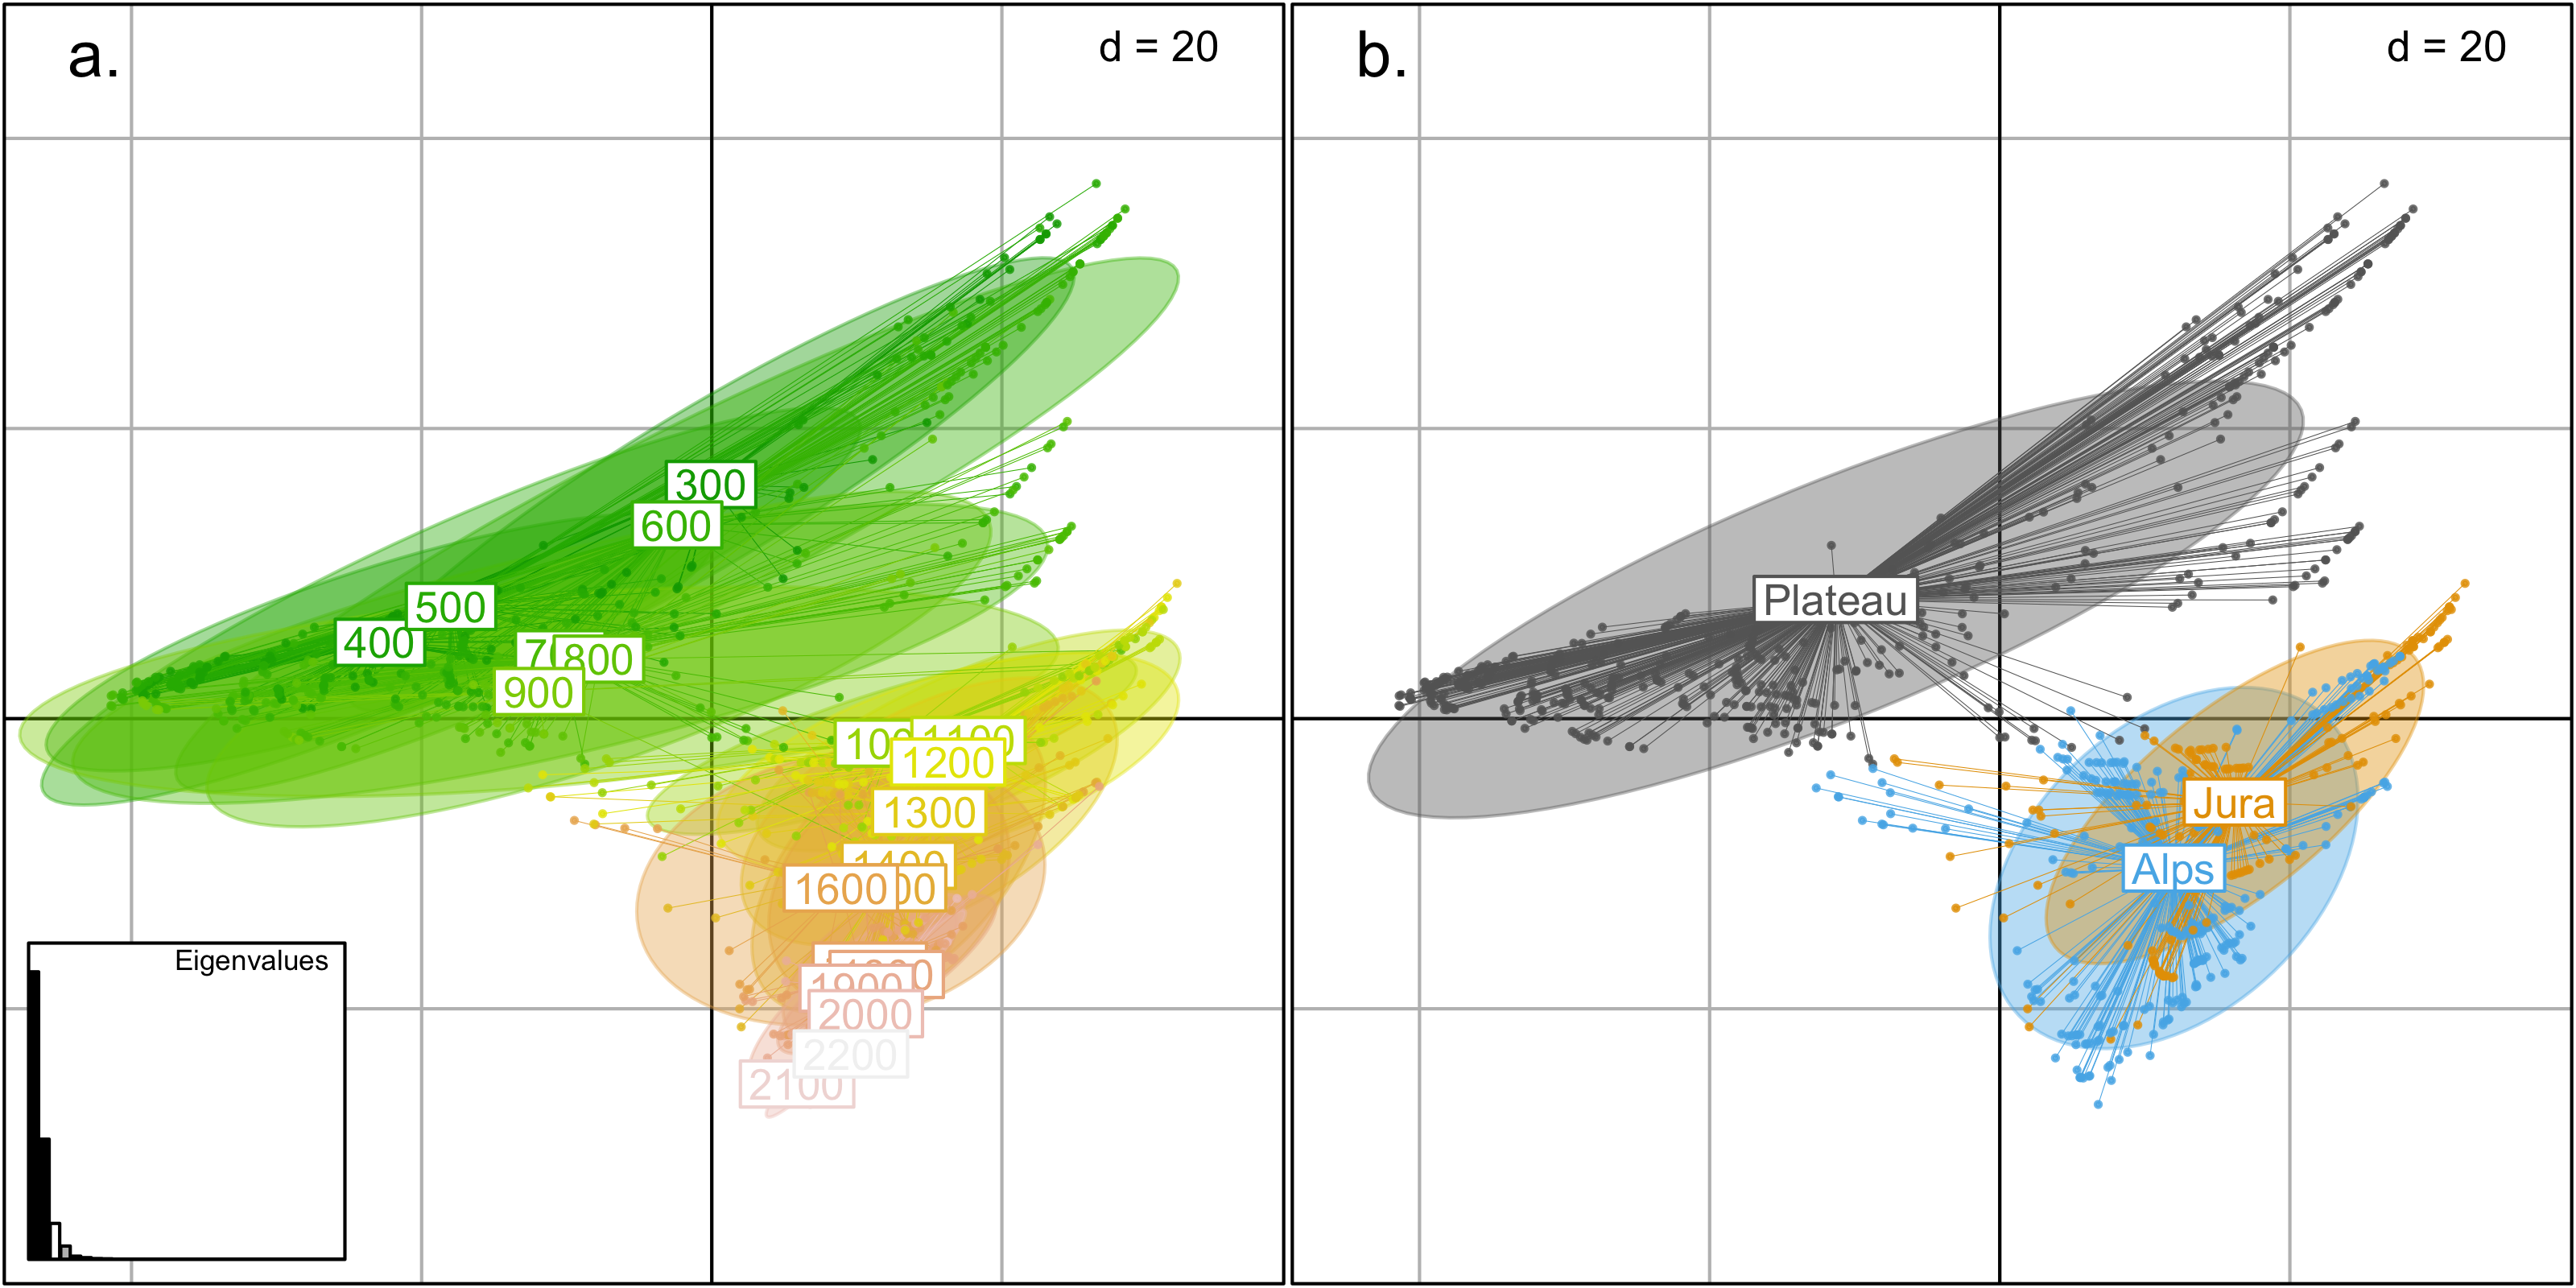
\includegraphics[width=5in]{ms/1_Ecography/1/figs/DPCoA.png}
	\caption{\label{fig:dpcoa} Double principle coordinate analysis (DPCoA) of local communities predicted by the \emph{Joint} model, with plots colored by (a) elevational bin, and (b) region. The central plateau includes hills from ~300m to ~1000m, with the Jura and the Alps rising steeply in the east and west, respectively. }
\end{figure}

Both the presence-only (\textbf{W}) and structured abundance (\textbf{Y}) datasets showed strong differences in the genus composition between the plateau and montane samples (Fig. \ref{fig:genus_assemblages}). In both datasets, the plateau ($<$1000m) was dominated by \emph{Lasius spp.}, with high representation of \emph{Formica spp.} in the montane zone ($\geq$1000m). The structured abundance dataset also showed high relative abundance of \emph{Myrmica spp.}, particularly in montane environments. Compared to the structured abundance dataset, the presence-only dataset under-represented 15 species (19\%) based on 95\% HPDIs (\textbf{Appendix 2 Fig}). Nine of those species were in the genus \emph{Myrmica}, which was particularly prevalent in the montane structured abundance samples. In contrast, only 3 species were over-represented, including the anthropophilic pavement ant \emph{Tetramorium immigrans}, and two species of large-bodied mound-building \emph{Formica}. 

\begin{figure}
	\centering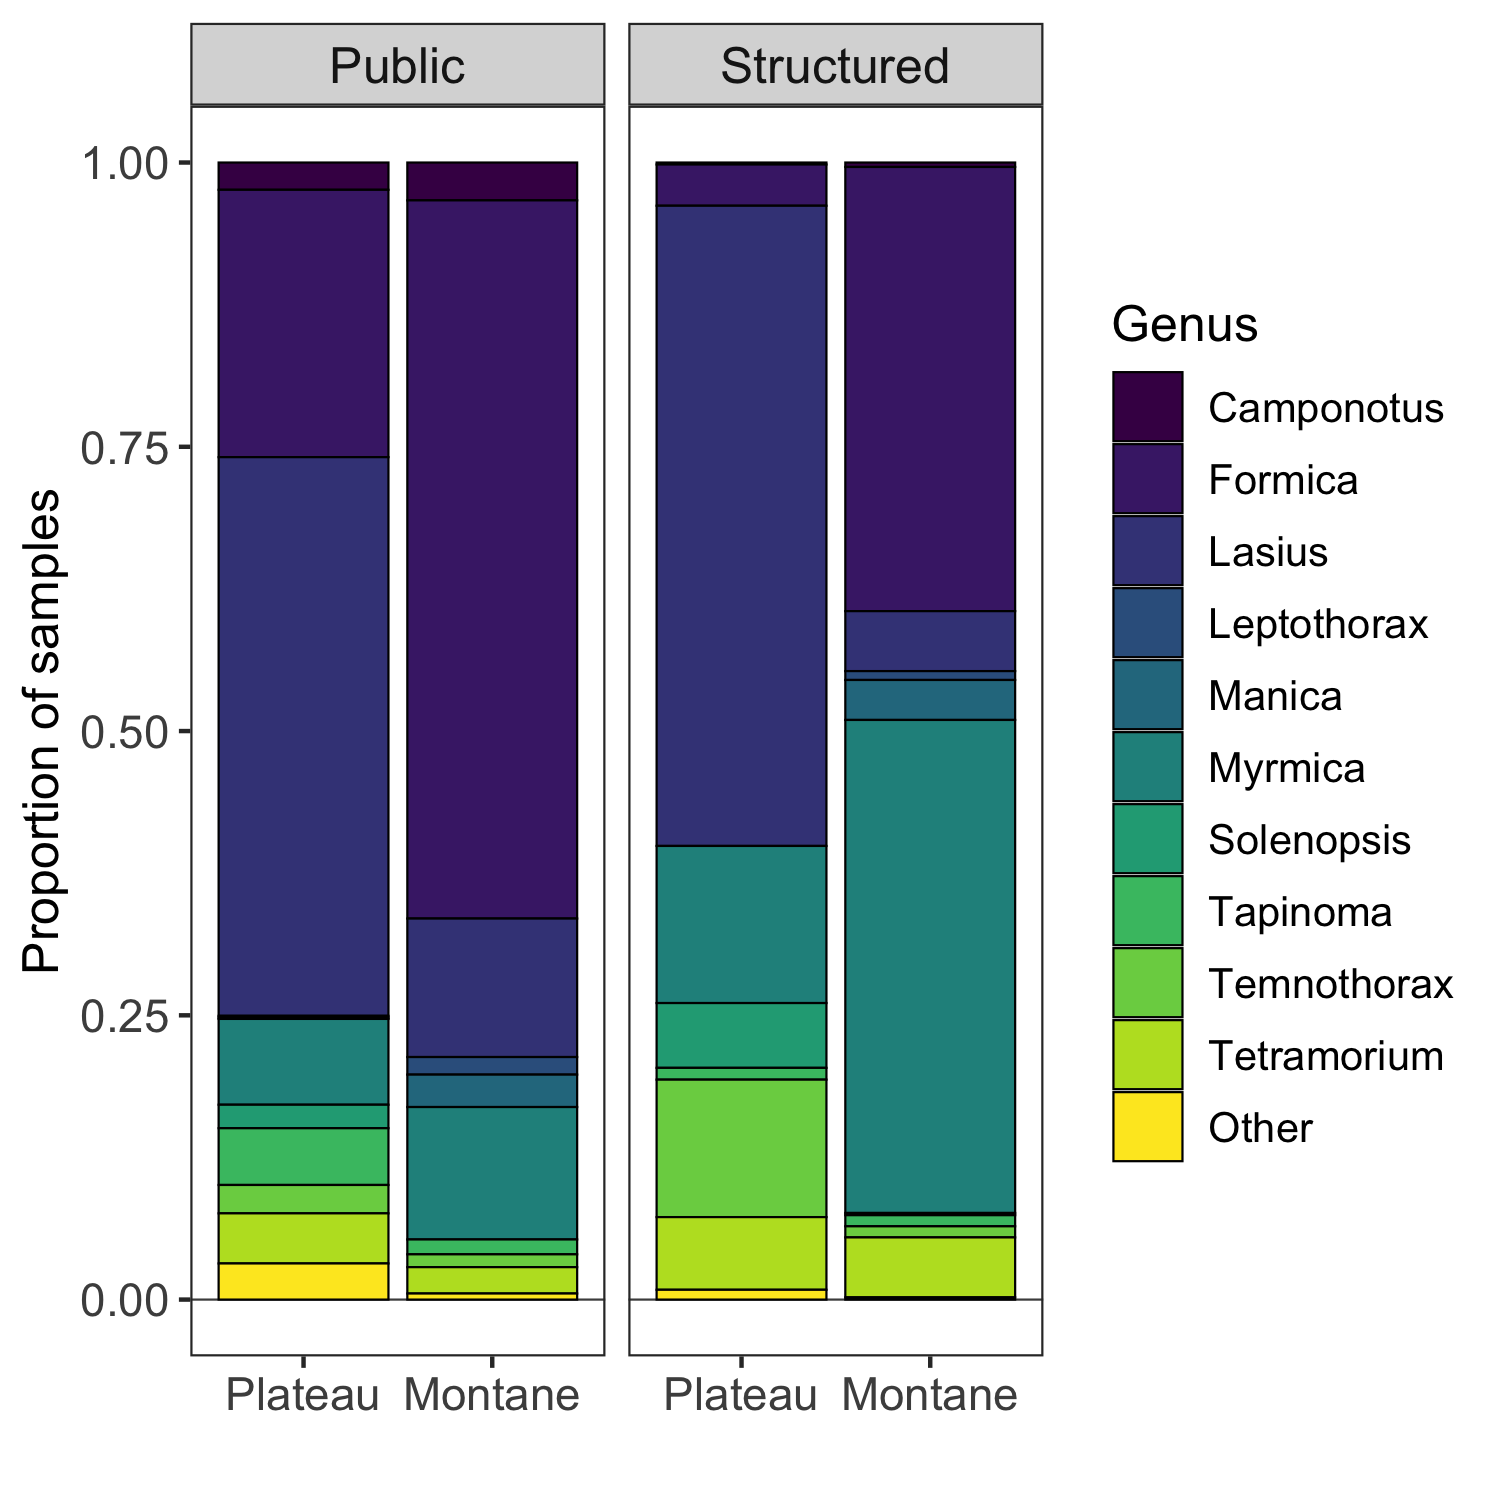
\includegraphics[width=3in]{ms/1_Ecography/1/figs/genus_assemblages.png}
	\caption{\label{fig:genus_assemblages} Genus composition in the presence-only and structured abundance datasets across plateau and montane environments. Only genera that constitute $\geq 1\%$ of at least one subset are shown, with others indicated as 'Other'.}
\end{figure}

Patterns of $\beta$-diversity and its components did not strongly differ between models (Fig. \ref{fig:beta_div}). Overall $\beta$-diversity among plots within each structured site decreased somewhat with elevation. At lower elevations, the variation among local plots was driven largely by the \emph{balanced variation} component, indicating changes in the relative intensity of species among plots. At higher elevations, the \emph{abundance gradient} component increased, indicating changes in total intensity among plots, with less variation in species' relative intensity. At the highest sites, the overall $\beta$-diversity was partitioned approximately equally between the two components.

\begin{figure}
\centering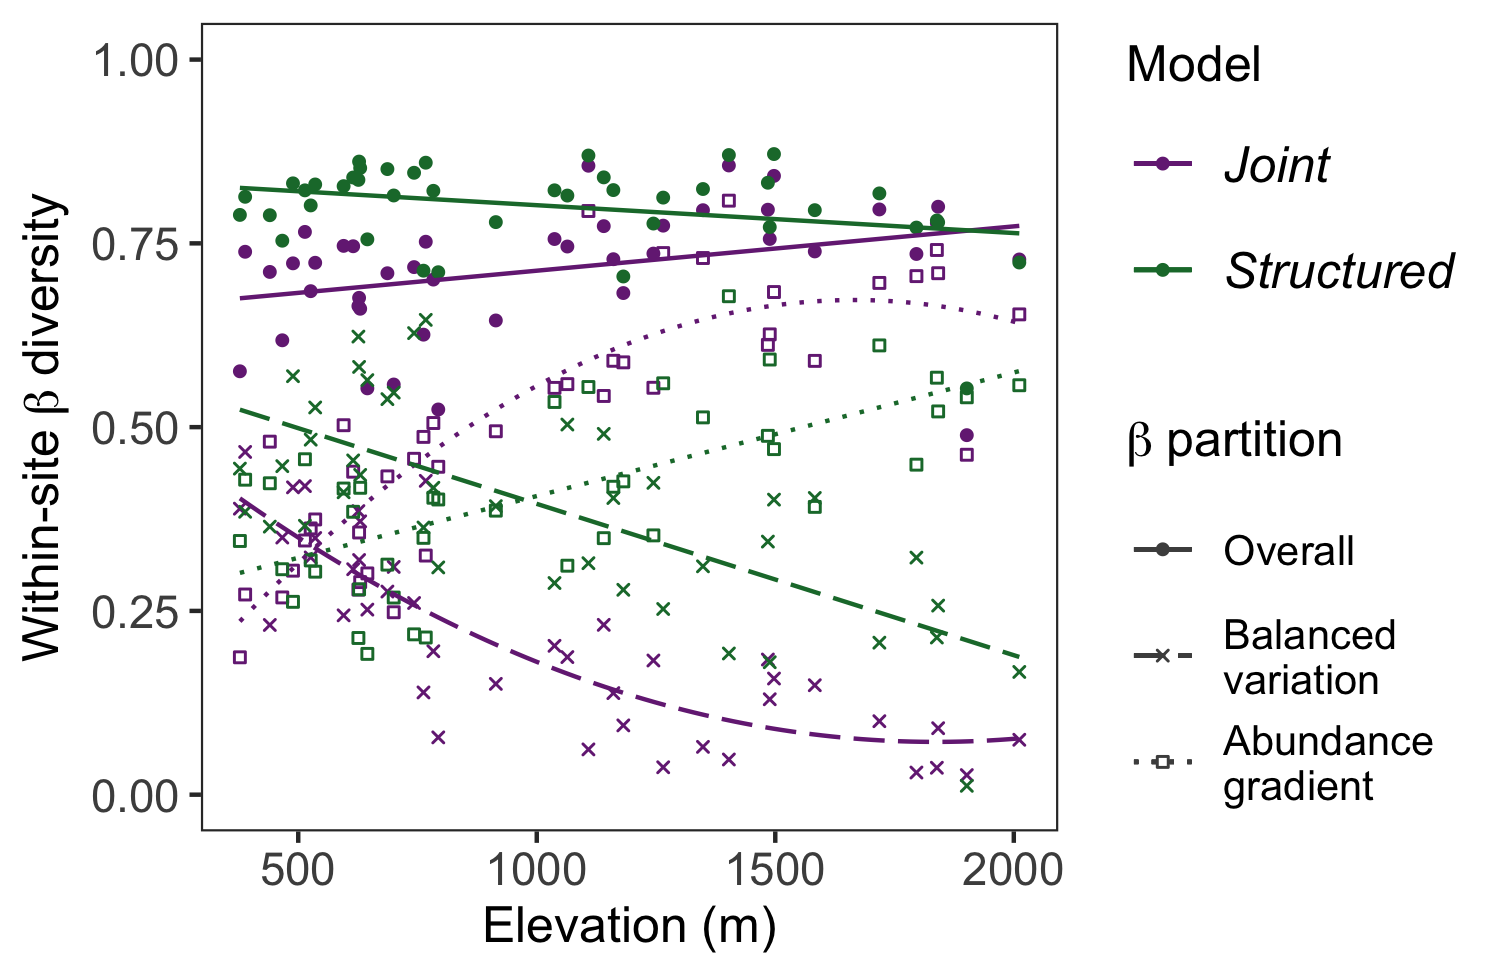
\includegraphics[width=3in]{ms/1_Ecography/1/figs/beta_diversity.png}
\caption{\label{fig:beta_div} Multi-site $\beta$-diversity and its components across elevation. Posterior medians were used to calculate multi-site $\beta$-diversity and its components within each 1 km$^2$ site, representing the variation among plots. \emph{Balanced variation} quantifies changes in relative abundance among species, while \emph{abundance gradient} denotes changes in total abundance.}
\end{figure}


 




\section{Discussion}
\label{S:4}
Citizen science papers: \citep{Altwegg2019, Pernat2020, Henckel2020, Duan2020, Johnston2020,Robinson2019, Beck2010, Poisson2020}

% Summary
The \emph{Joint} model outperformed the \emph{Structured} model, indicating that the information provided by the presence-only dataset at a regional scale improved predictions of ant communities at a local scale as well. Further, the \emph{Joint} model reduced uncertainty in species-level responses at both spatial scales, and for species detected or undetected in the structured abundance dataset. At a regional scale, ant richness was predicted to increase somewhat through the Swiss plateau, peak at the base of the mountain ranges, and then decline with further increases in elevation. In contrast, Shannon diversity was predicted to decline from low elevations until the mountain base, and then remain steady. Patterns were best predicted by growing degree days, precipitation, forest cover, and road length at a regional scale, and soil temperature, canopy cover, and crop or pasture land use at a local scale. Local ant communities cluster into plateau and montane communities, with large differences in the relative abundance of genera across elevations. At low elevations, the variation among local communities is dominated by variation in relative abundance among species, while at high elevations it is equally determined by variation in relative abundance and total abundance.

% Patterns
Divergent patterns at a local vs. regional scale. Seems like there's some density compensation. Uncertainty is large at high elevations, partly due to extrapolation beyond the soil plots, and partly due to some of the species at higher elevations that occur at high densities and form super colonies. Richness, diversity, and total intensity all tell somewhat different stories. Square kilometers are also pretty large, and particularly in the mountains can include a fairly large elevational range. They also don't take into account things like species interactions (though I'm skeptical that they actually scale up to a 1 km2) or stochastic variation in actual occupancy of available habitats. At the regional scale, the intensities are somewhat more about the potential occurrence I think. For example, the regional predictions don't directly take into account the amount of cropland, which clearly has a large negative effect on basically all species. If such data had been available, it likely would have improved predictions, and led to lower predictions.

% Supported drivers
Paragraph on supported environmental drivers. Temperature preferences vary a lot between species. So do canopy effects. Crop is universally bad, pasture is mostly good. Local soil temperature is mostly good. 

% Assemblages
Paragraph on assemblages. There's some work that supported this, but it's not the most common thing to find based on my memory. But in these ants it's pretty clear that the communities cluster into plateau and montane assemblages. However, this distinction is driven by a minority of species; 51\% of species were detected in both the plateau and the montane, with 34\% restricted to the plateau and 15\% exclusively montane. Thus, while the local communities can be clearly distinguished, that does not mean they are entirely distinct. Given the differences between the Jura and the Alps (which are what?), it's maybe a little surprising to not really see any differentiation. On the other hand, how determined are these lambdas by the environment? If the regional and local variables don't show much differentiation between the two mountain ranges, then the lambdas wouldn't either... I could add a PCA of the environmental variables to the appendix. But even so, there's nothing in the model that forces the communities to separate cleanly by elevation. That's a reflection of the data. I should also add an appendix figure of the elevational range of each species. There's also more local variation in the species composition at lower elevations, meaning more variation in the expected species identities across plots. 

% Hierarchical shrinkage and rare species
Somewhere, I should talk about hierarchical shrinkage, and how the model estimates species' responses in situations where occurrences are limited. This is true for both models, but is particularly important in the \emph{Structured} model, where there are some species that were not detected, but were nonetheless included in the model. As implemented here, the method of hierarchical shrinkage assumes that, in the lack of additional data, a species is likely to respond to environmental variables in a manner similar to its congeners. If there are no congeners (or no congeners with data), then a species is likely to respond in a manner similar to a generic ant, based on the aggregate responses. This is true for the relative intensities across the landscape. However, the absolute intensity is still informed by the lack of observations in the structured samples. That is, undetected species are likely to be rare. This explains some of the differences in species-level and genus-level responses between the two models. For example, very few \emph{Camponotus} were detected in the structured samples (\textbf{APPENDIX 2 TABLE SX}) because they don't nest in the soil, and so the structured plots were unlikely to include a tree that served as a nest. Consequently, the richness for the genus predicted by the \emph{Structured} model is generally low, and the relative pattern is informed by the aggregate ($\beta$) responses as well as the few detections of \emph{C. ligniperdus} (Fig. \ref{fig:gen_map_Structured}, \ref{fig:b_byParam}). The pattern predicted by the \emph{Joint} model is rather different, because the preferences of these species are further informed by the occurrences from the presence-only dataset (Fig. \ref{fig:gen_map_Joint}, \ref{fig:b_byParam}). Thus, given a paucity of information on a species, the use of taxonomic hierarchical shrinkage provides a 'best guess' based on other species, with greater weight on closely related species, and with appropriately larger uncertainty (Fig. \ref{fig:slope_means}, \ref{fig:b_byParam}).

% Bias in citizen science data
The sampling was definitely spatially biased, such that many cells only had one sample, and a few cells had hundreds. The taxonomic composition was not in line with the taxonomic composition of the structured samples, which more accurately quantified colony density. There was more of a tendency to under-represent species than over-represent species, particularly those that have somewhat less obvious lifestyles like \emph{Myrmica}, some \emph{Lasius}, and some \emph{Temnothorax}.  

% Value in citizen science data
Paragraph on what the citizen science data contributes. Very broad spatial coverage, despite unevenness. Inclusion of rarer species that are unlikely to be detected in a structured survey focused on colony density. Reduced uncertainty in species' responses to both local and regional variables, including for species detected in the structured abundance dataset. Better out-of-sample predictive ability for local abundances. How does this fit with the other handful of recent studies about using citizen science data?

% Conclusion
Conclusion



\section{Acknowledgments}
Thanks to everyone.

\newpage
\section{Bibliography}
\bibliography{ms/opfo_diversity}



\newpage
\section{Appendixes}
\textbf{Appendix 1. Supplementary methods.}
\begin{enumerate}
    \item Further description of the sampling?
    \item Figure of grid with number of samples?
    \item Table of covariate information
    \item Table of land cover types and canopy classification
    \item Table of parameters?
    \item Further description of the model?
    \item Prior distributions
    \item Model code
\end{enumerate}

\begin{table}[ht]
	\centering
	\begin{tabular}{ l l c }
		\hline
		\textbf{Parameter} & \textbf{Description} & \textbf{Type} \\
		\hline
		$i$ & structured sampling plots (0.75 m$^2$) & index \\
		$j$ & structured sampling cells (1 km$^2$) & index \\
		$k$ & citizen science cells (1 km$^2$) & index \\
		$s$ & species & index \\
		$g$ & genus & index \\
		$l$ & local covariates (0.75 m$^2$) & index \\
		$r$ & regional covariates (1 km$^2$) & index \\
		\hline
		$\mathbf{Y}_{is}$ & structured sampling counts (0.75 m$^2$) & data \\
		$\mathbf{W}_{ks}$ & citizen science counts (1 km$^2$) & data \\
		$\mathbf{V}_{il}$ & local covariates (0.75 m$^2$) & data \\
		$\mathbf{X}_{(jk)r}$ & regional covariates (1 km$^2$) & data \\
		$h$ & structured sampling proportional effort & data \\
		\hline
		$\mathbf{\lambda}_{is}$ & colony intensity (0.75 m$^2$) & latent \\
		$\mathbf{\Lambda}_{(jk)s}$ & colony intensity (1 km$^2$) & latent \\
		\hline
		$\alpha_{l}$ & aggregate ant responses (0.75 m$^2$) & slopes \\
		$\mathbf{A}_{lg}$ & genus-level ant responses (0.75 m$^2$) & slopes \\
		$\mathbf{a}_{ls}$ & species-level ant responses (0.75 m$^2$) & slopes \\
		$\sigma^a_{l}$ & response sd among congeners & sd \\
		$\mathbf{\Sigma^A}_{gg}$ & genus-level covariance matrix & cov mx \\
		$\beta_{r}$ & aggregate ant responses (1 km$^2$) & slopes \\
		$\mathbf{B}_{rg}$ & genus-level ant responses (1 km$^2$) & slopes \\
		$\mathbf{b}_{rs}$ & species-level ant responses (1 km$^2$) & slopes \\
		$\sigma^b_{r}$ & response sd among congeners & sd \\
		$\mathbf{\Sigma^B}_{gg}$ & genus-level covariance matrix & cov mx \\
		$D_{s}$ & citizen science species bias (proportional) & random effect \\
	\end{tabular}
	\caption{\label{table:params} Parameters in the model. Could be moved to an appendix, or shortened since many of these don't need to be highlighted. }
\end{table}

\textbf{Appendix 2. Supplementary results.}
\begin{enumerate}
    \item Table of species, with taxonomic info and total counts (or elevational bins?) for each dataset
    \item Table of variable selection loo
    \item Figure of species-level responses (points + HPDIs)
    \item Figure of species-level responses (bar proportions)
    \item Figure of taxonomic bias
    \item Figure of plateau vs montane species' intensities
    \item Covariance or sd for slopes?
    \item Maps of richness (total, by SF, by genus)
\end{enumerate}

\begin{figure}
	\centering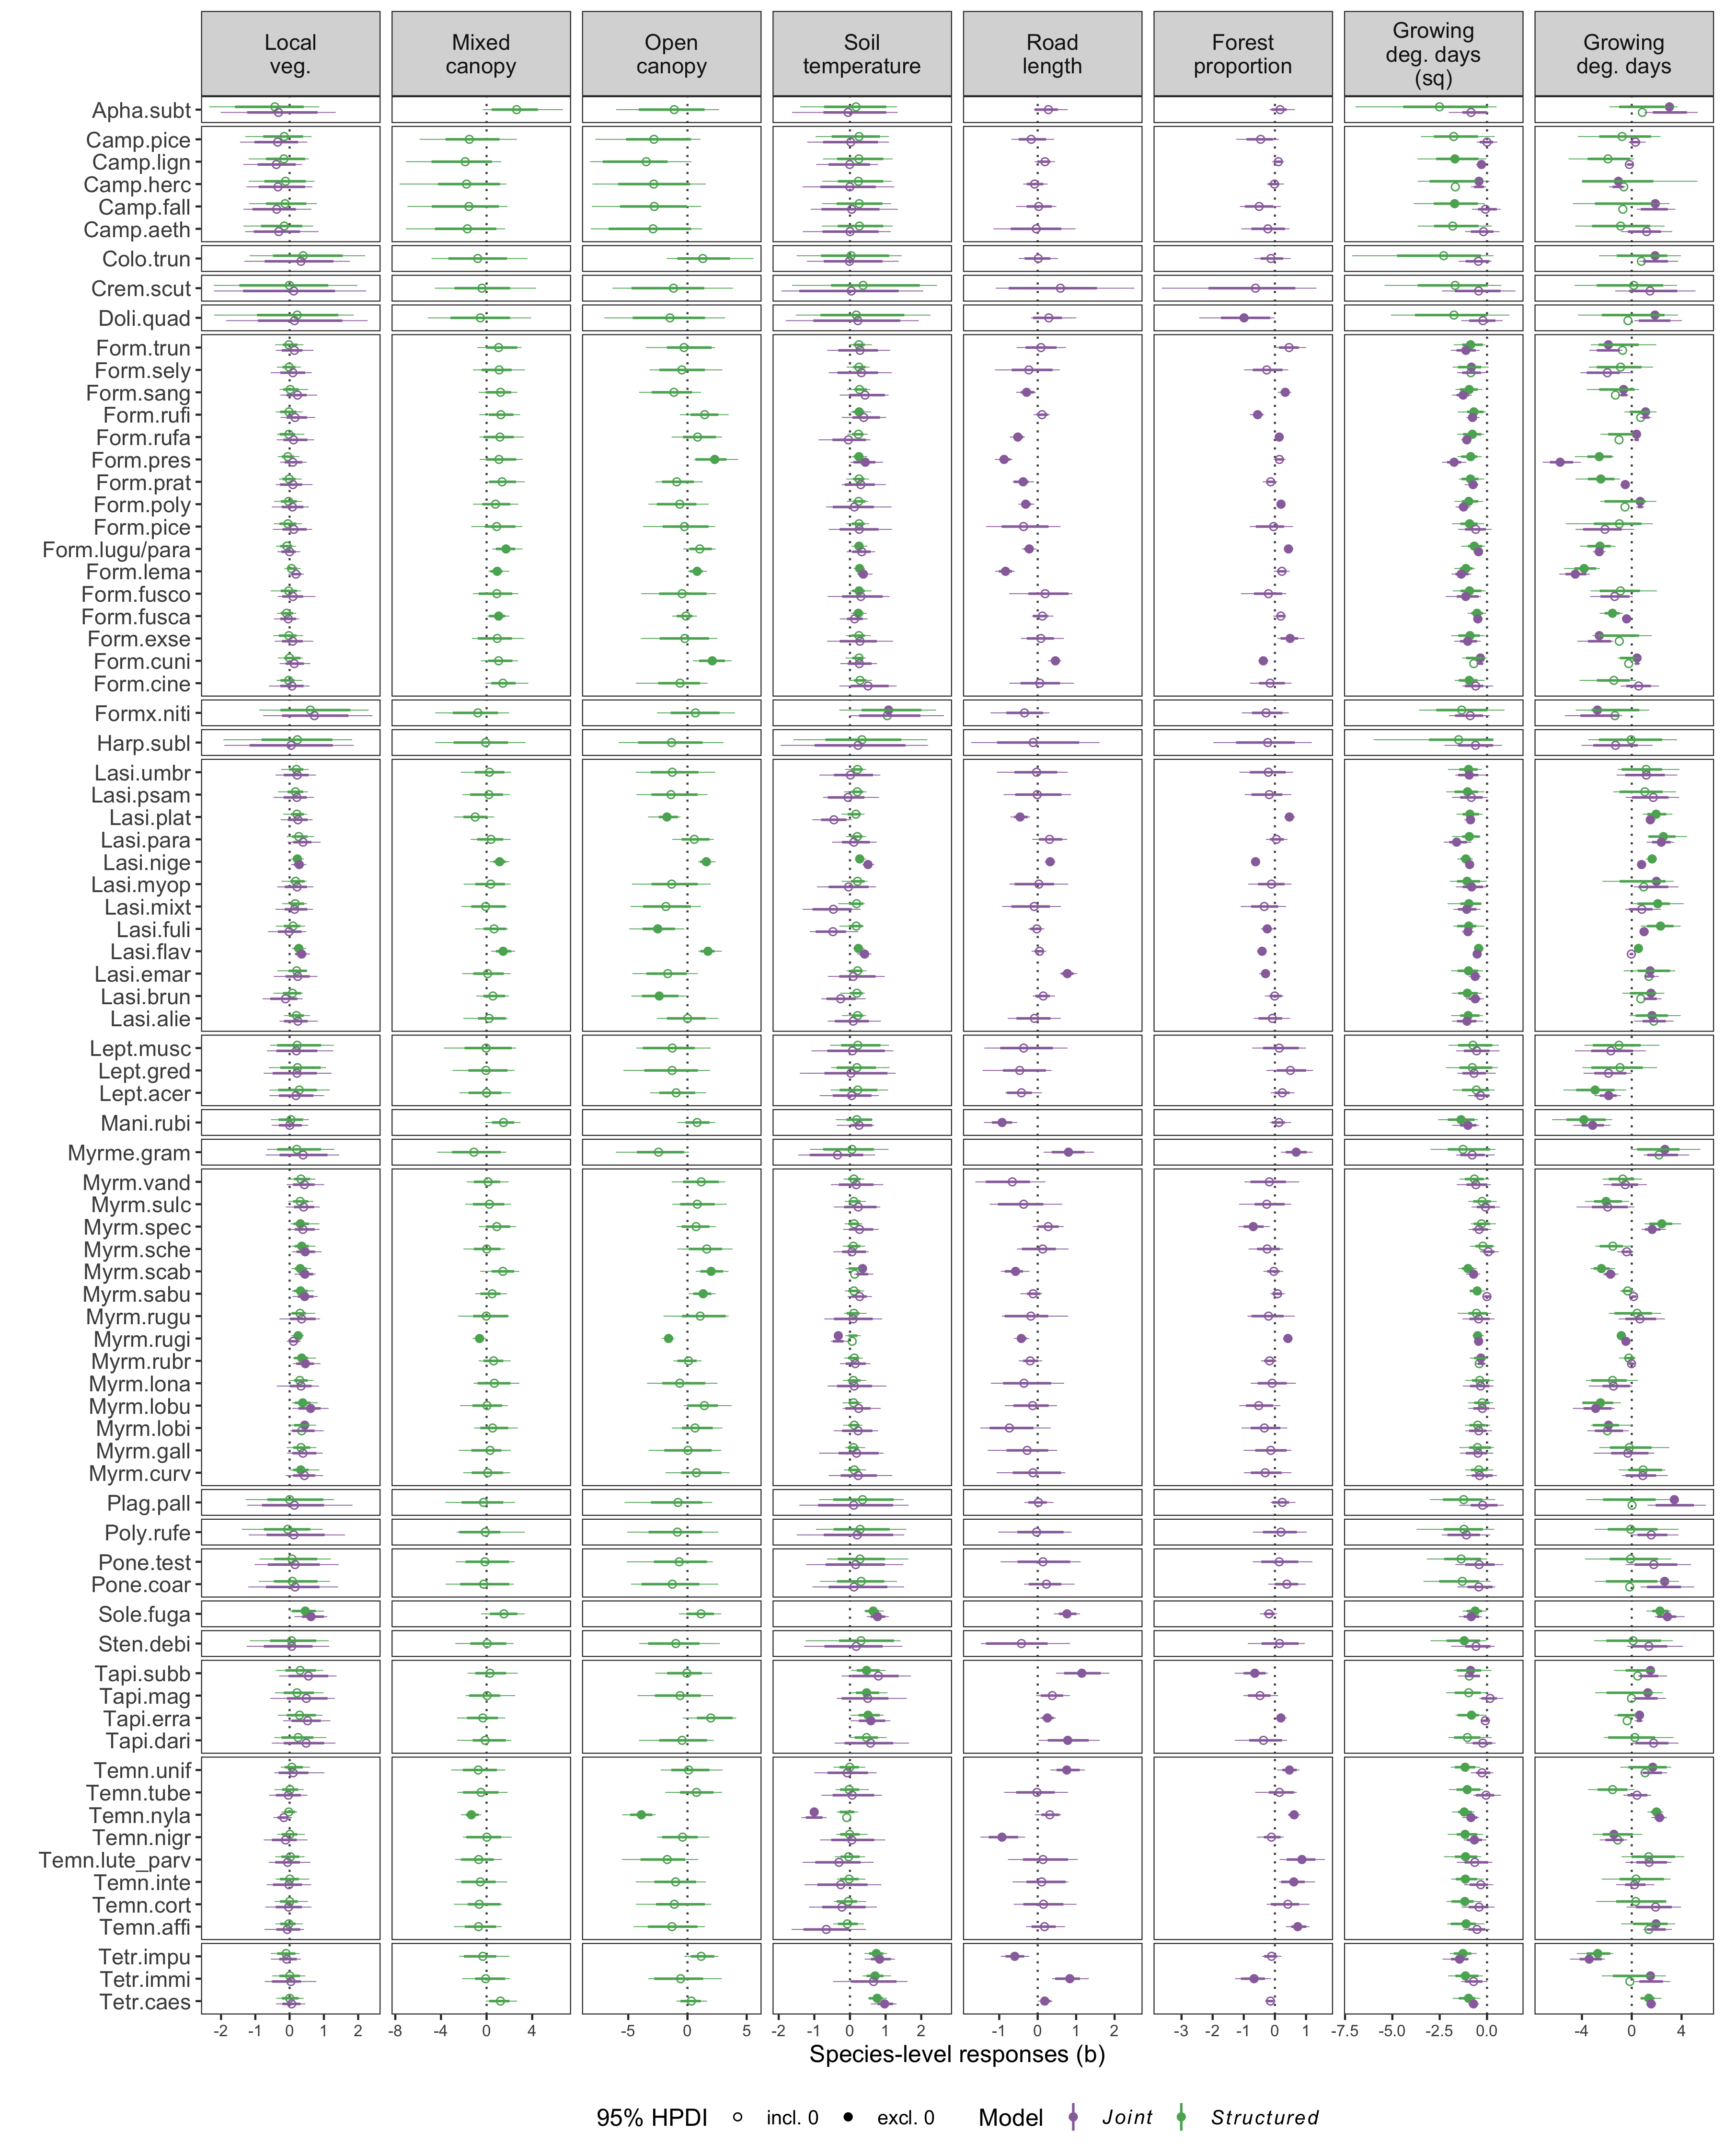
\includegraphics[height=7.5in]{ms/1_Ecography/1/figs/b_opt_byParam.png}
	\caption{\label{fig:b_byParam} Posterior species responses to local and regional covariates. Points show posterior medians, while bars show the Highest Posterior Density Intervals (HPDIs: 80\%: thick; 95\%: thin). Solid points indicate 90\% HPDIs that exclude zero in the \emph{Joint} (purple) and \emph{Structured} (green) models.}
\end{figure}

\begin{figure}
	\centering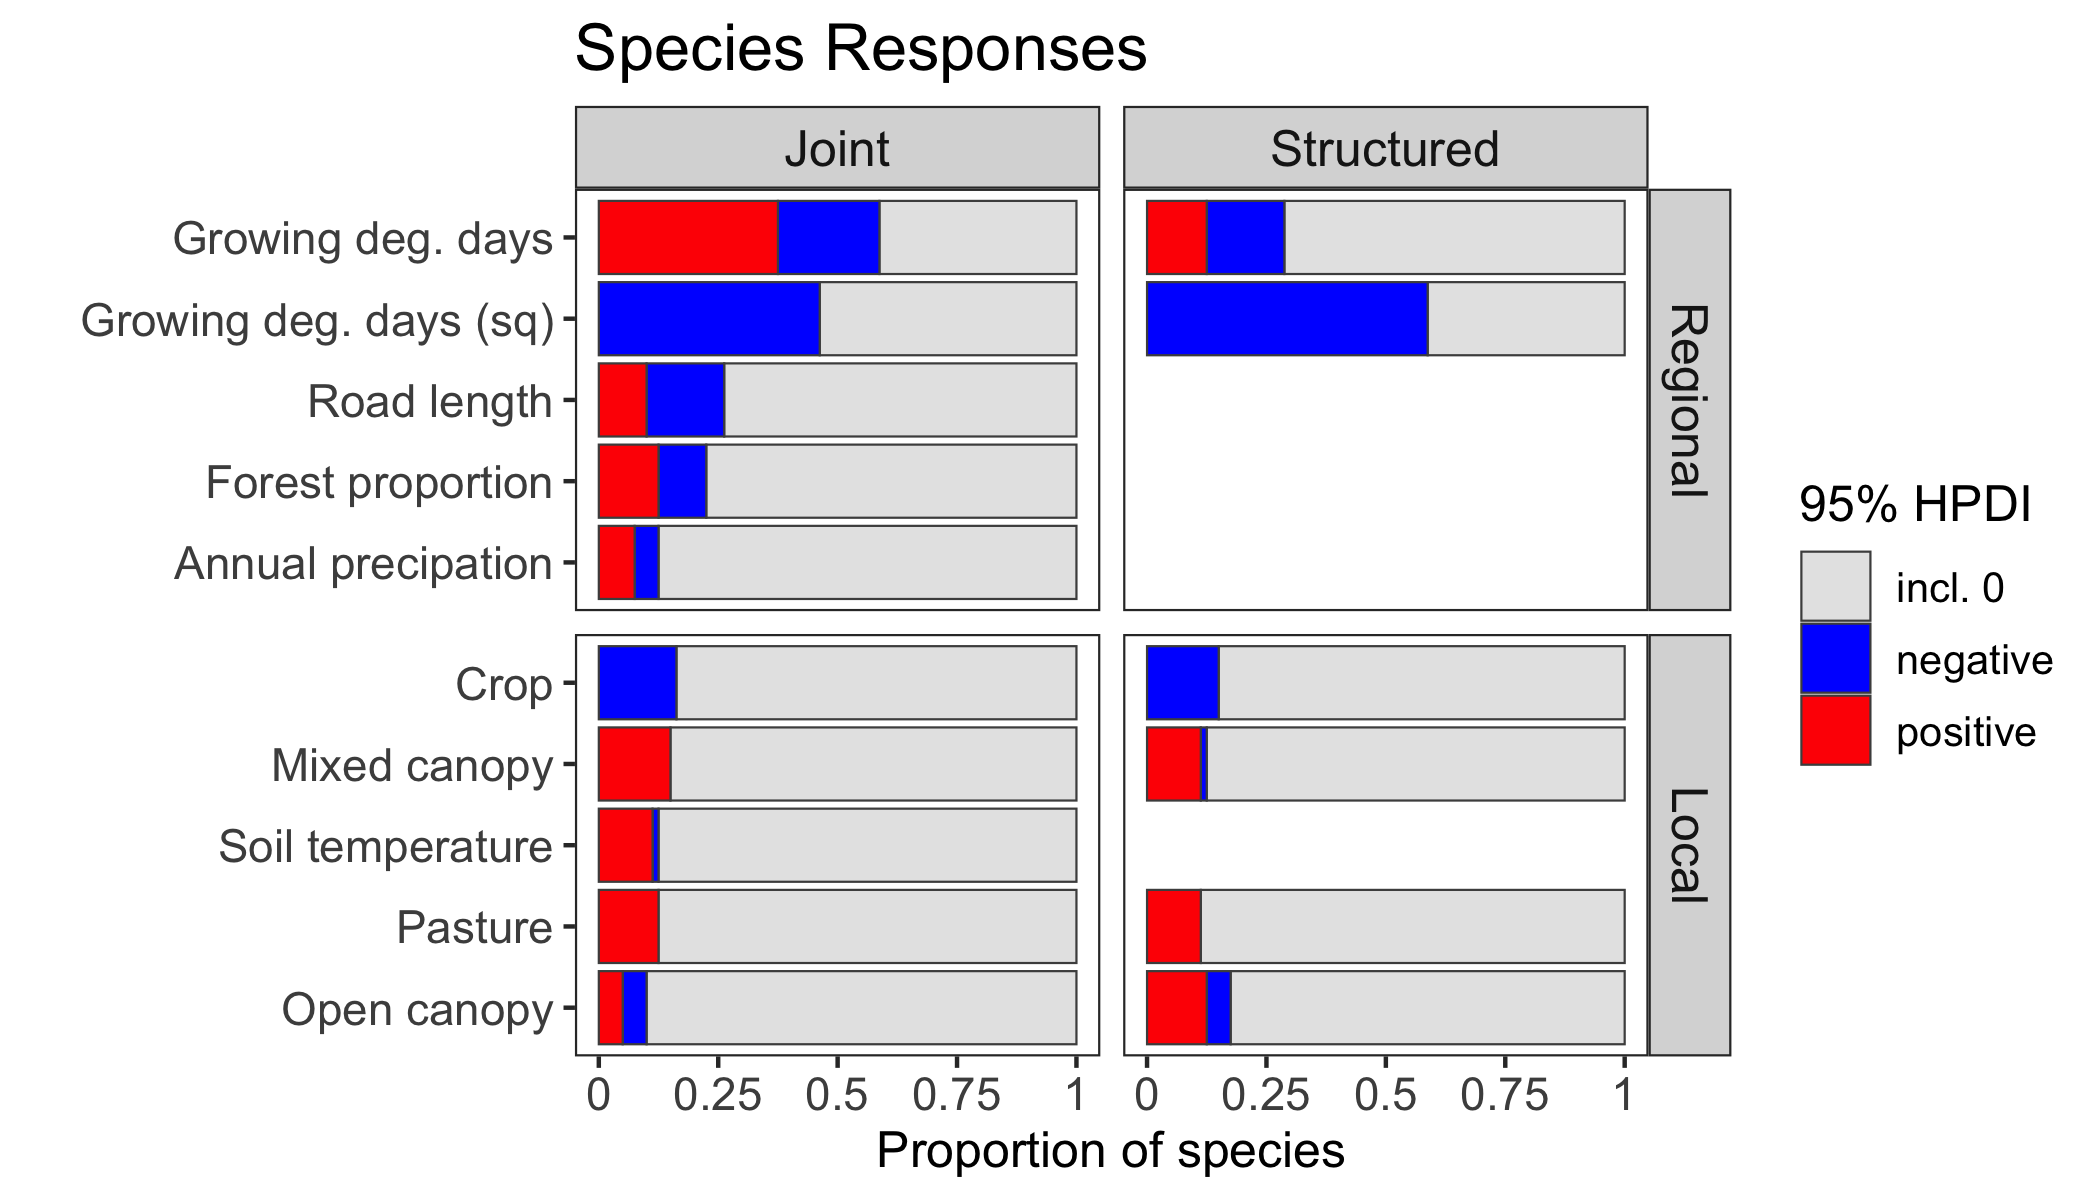
\includegraphics[width=6.5in]{ms/1_Ecography/1/figs/b_opt_bar.png}
	\caption{\label{fig:b_bars} Proportion of species' responses to each covariate. Responses are considered positive (red) or negative (blue) if the Highest Posterior Density Interval (HPDI) excludes zero for (a) 95\% HPDIs and (b) 80\% HPDIs. }
\end{figure}

\begin{figure}
	\centering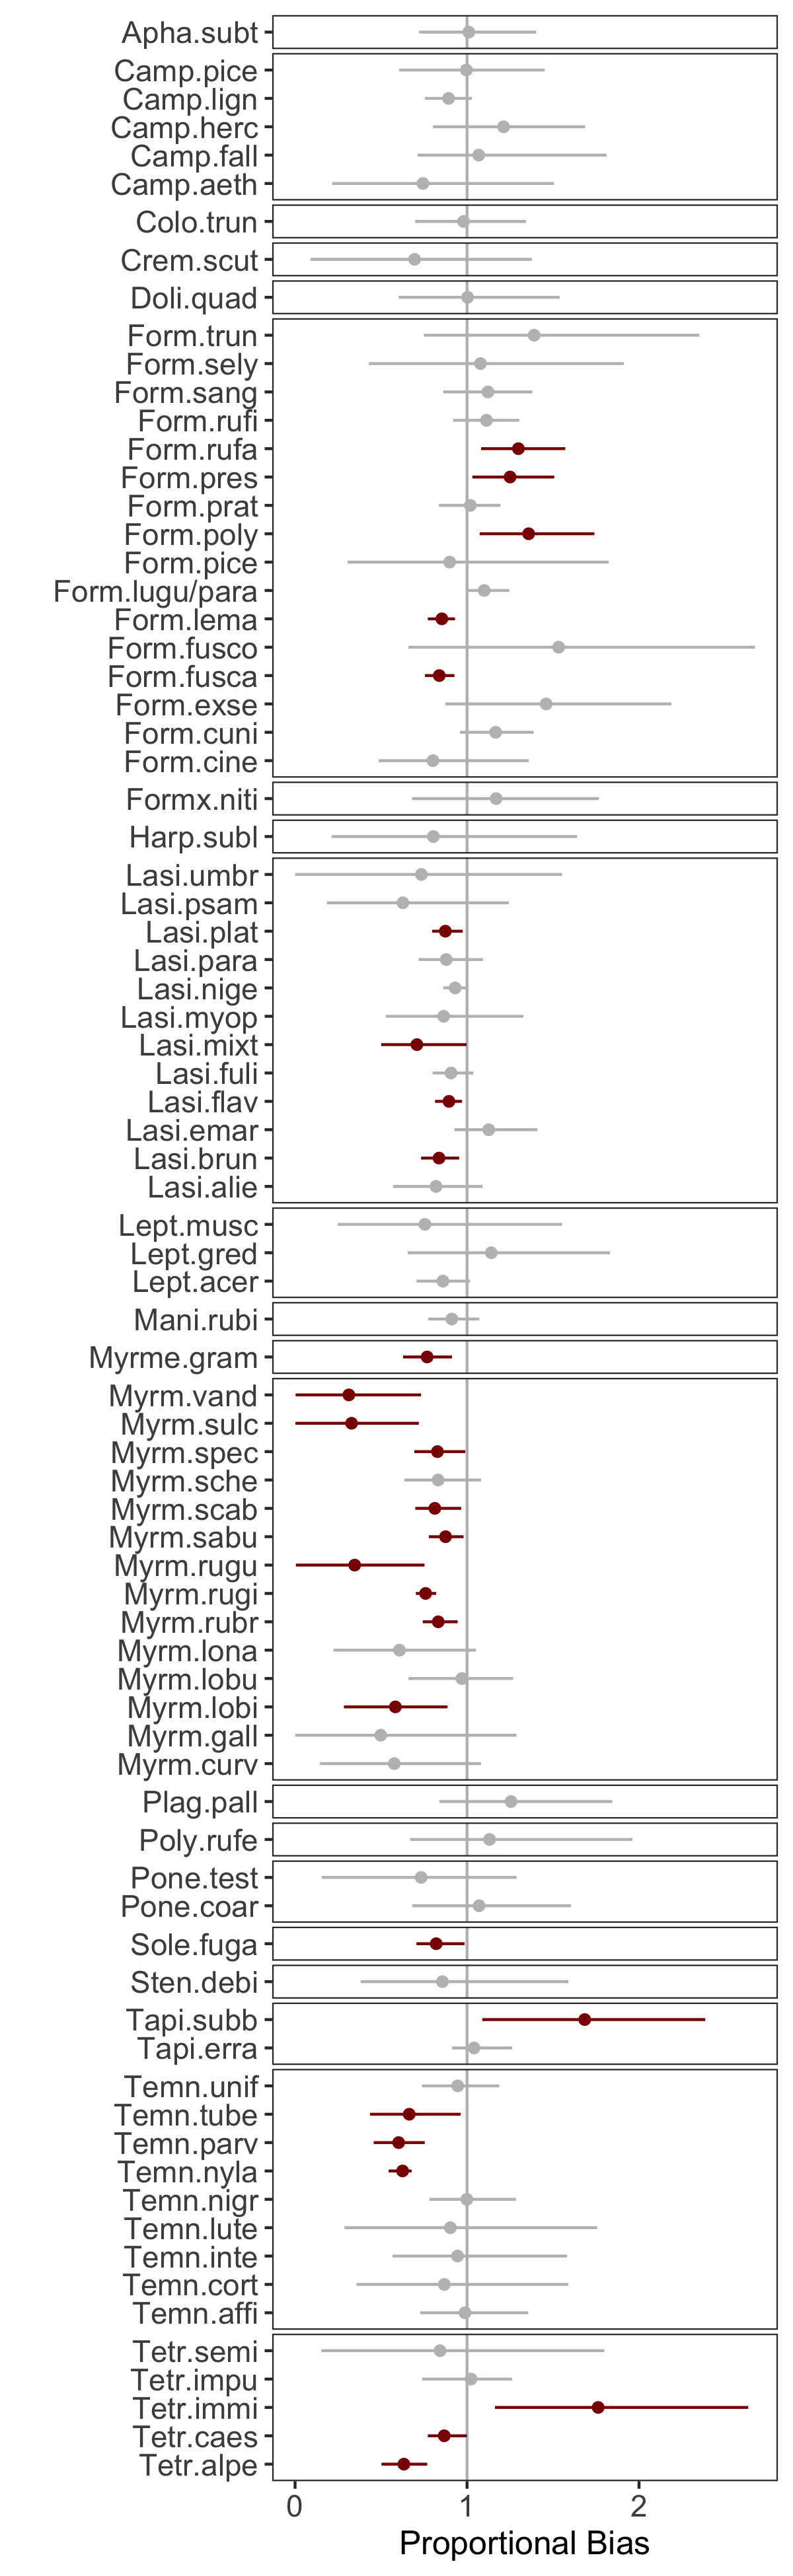
\includegraphics[height=8in]{ms/1_Ecography/1/figs/D_opt.png}
	\caption{\label{fig:D} Proportional taxonomic bias posterior distributions. Medians and Highest Posterior Density Intervals (HPDIs; 80\%: thick; 95\%: thin) for the representation of each species in the presence-only dataset relative to the structured abundance dataset. Values less than 1 indicate under-representation in the presence-only dataset. Dark red: 95\% HPDIs exclude zero; light red: 80\% HPDIs exclude zero. }
\end{figure}

\begin{figure}
	\centering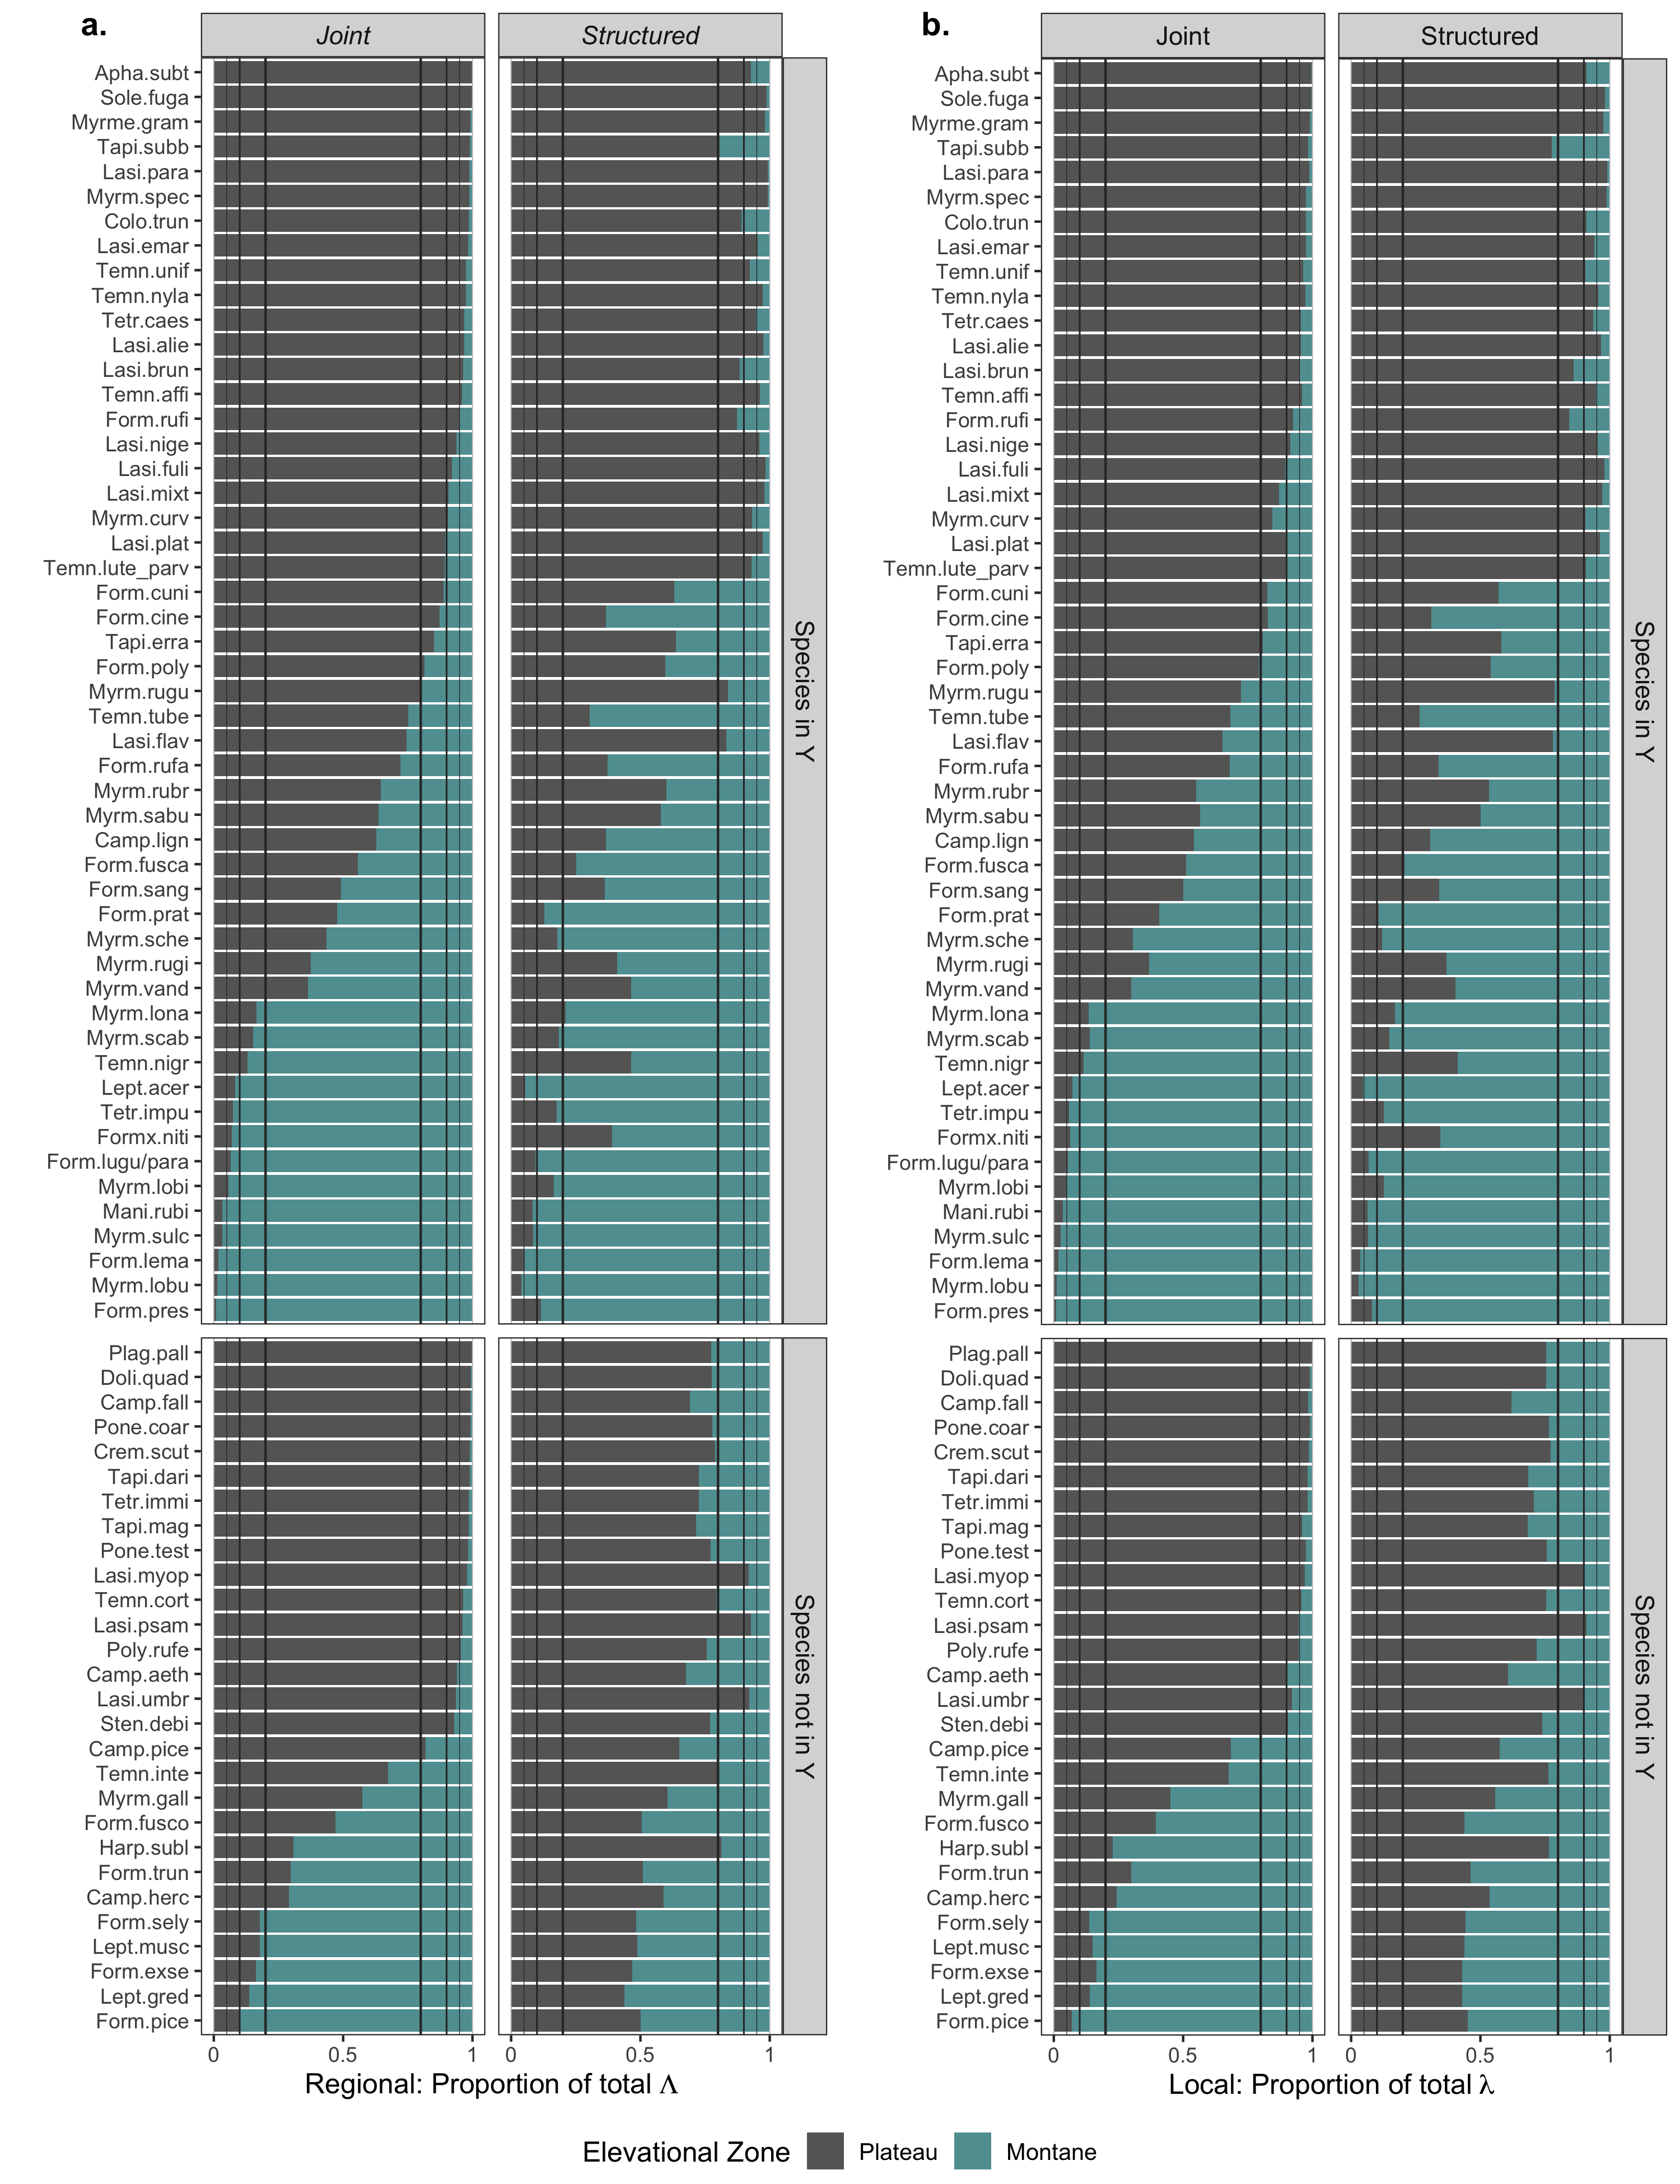
\includegraphics[height=8in]{ms/1_Ecography/1/figs/lambda_zones.png}
	\caption{\label{fig:lam_zones} Posterior species intensity across plateau and montane zones in the \emph{Joint} and \emph{Structured} models. Each species' total intensity (a. Regional; b. Local) was partitioned into the proportion occurring in the plateau ($<$1000m: grey) and montane ($\geq$1000m: green) zones. Vertical lines indicate 80\%, 90\%, and 95\% for either zone. }
\end{figure}

\begin{figure}
	\centering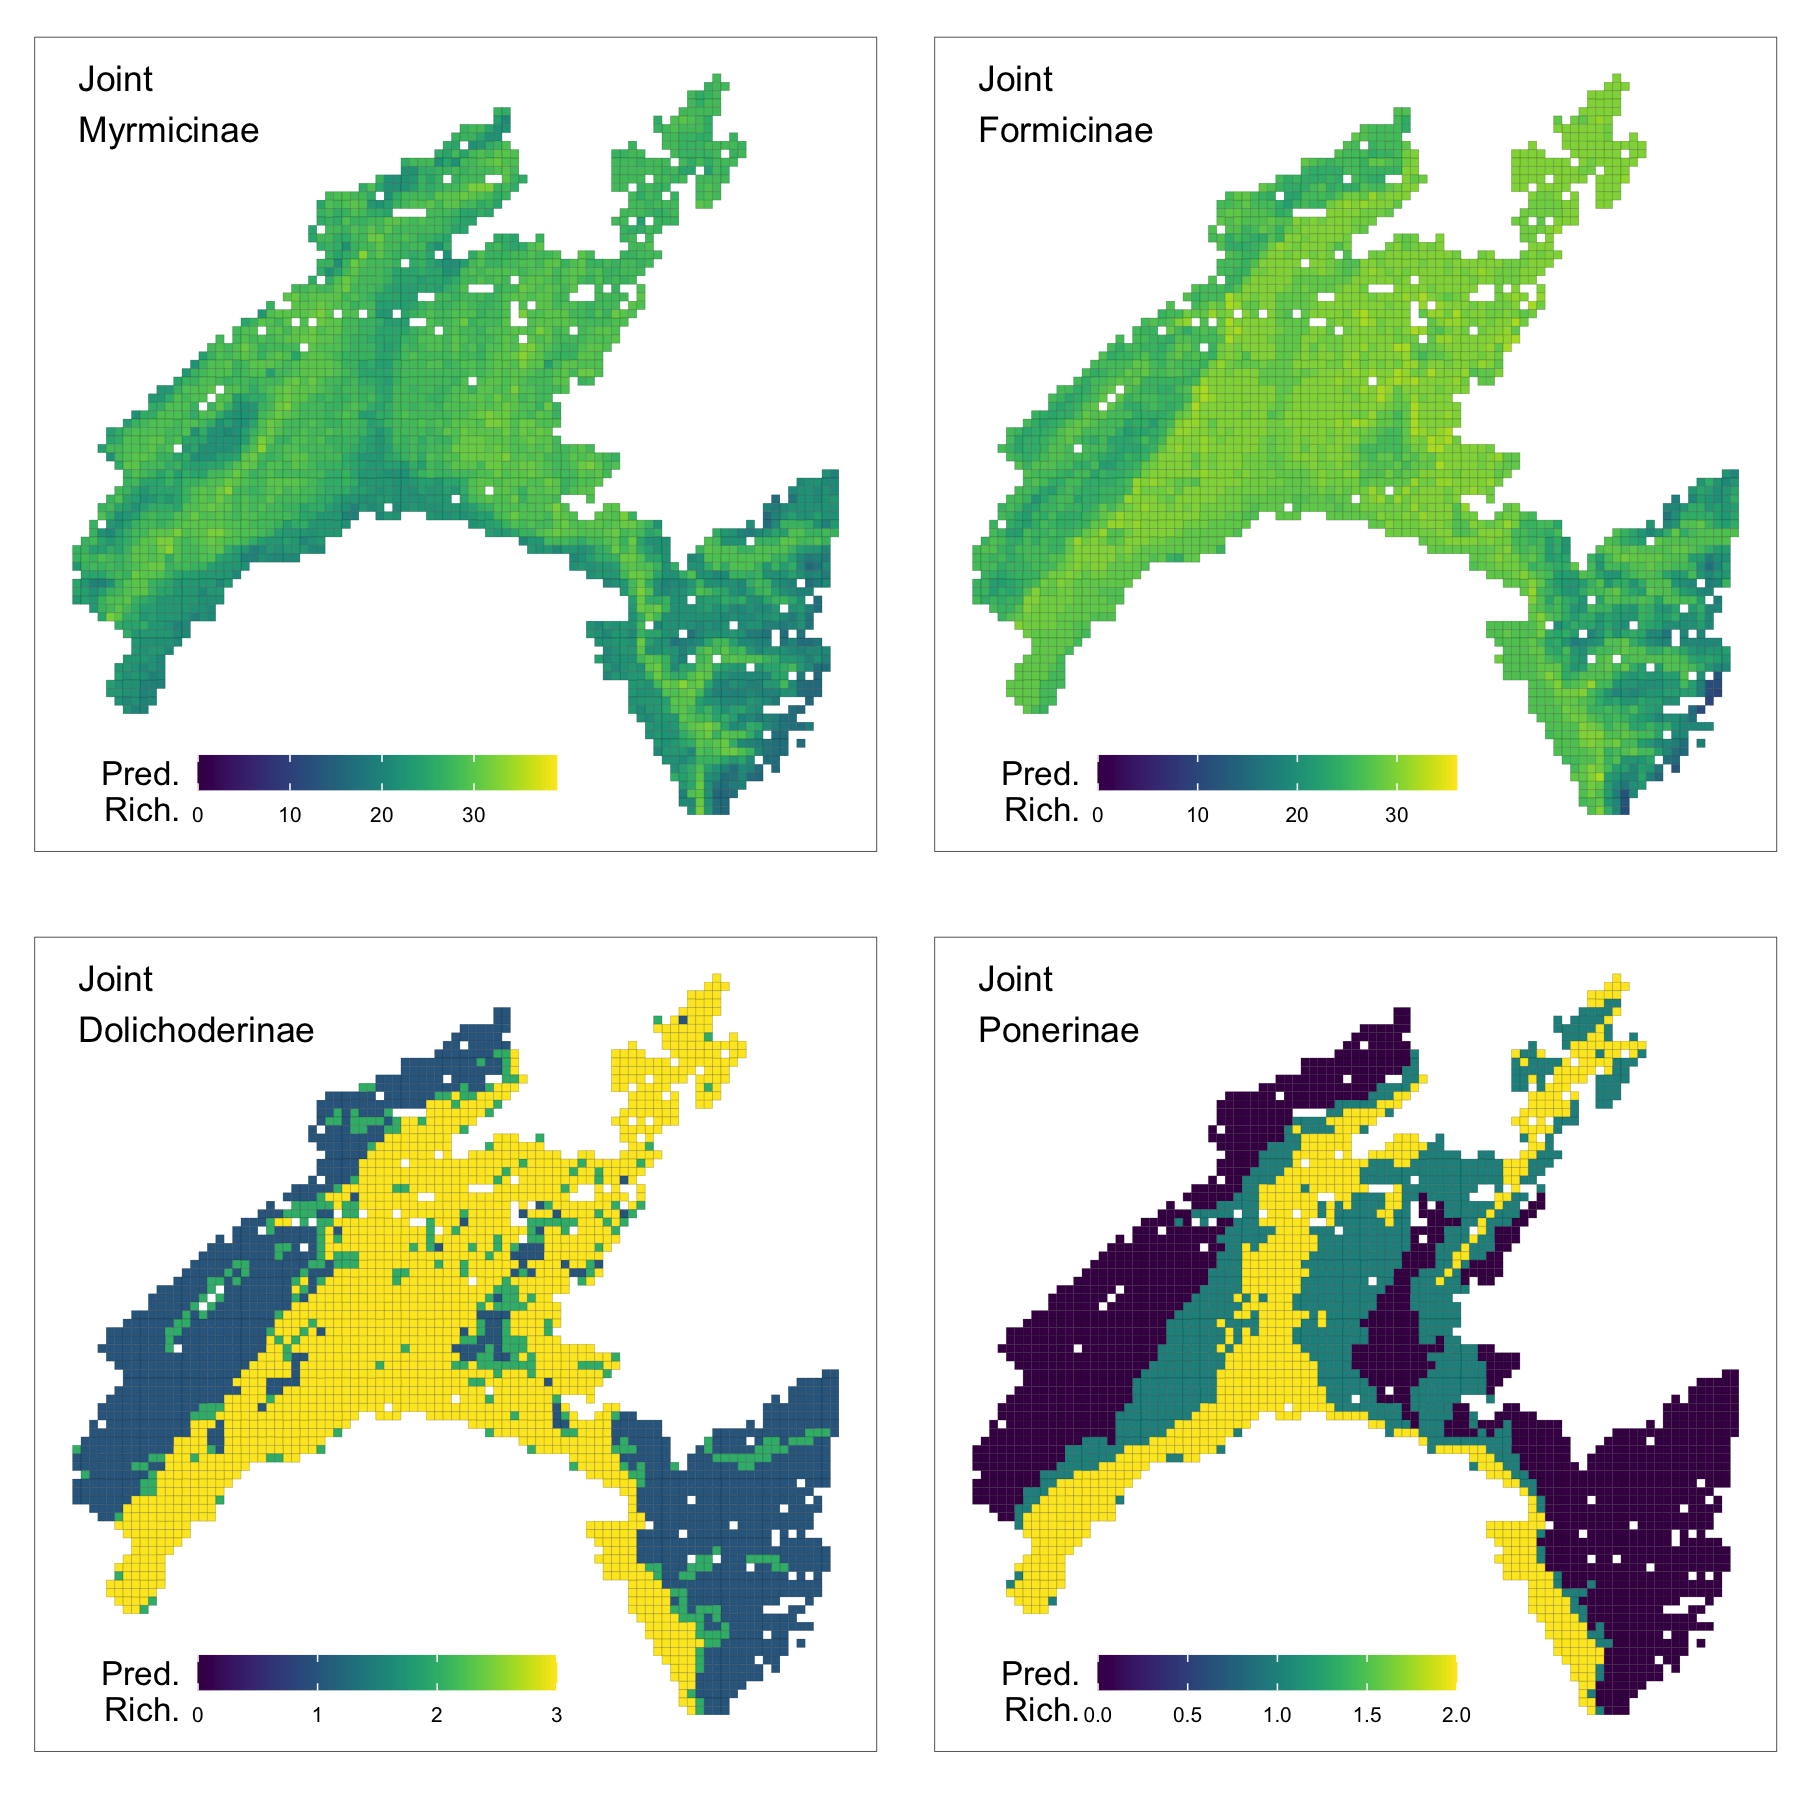
\includegraphics[width=5in]{ms/1_Ecography/1/figs/maps/sf_S_WY.png}
	\caption{\label{fig:sf_map_Joint} Maps of predicted richness in the \emph{Joint} model for subfamilies. Predictions are based on 95\% Highest Posterior Density Intervals for each species. }
\end{figure}

\begin{figure}
	\centering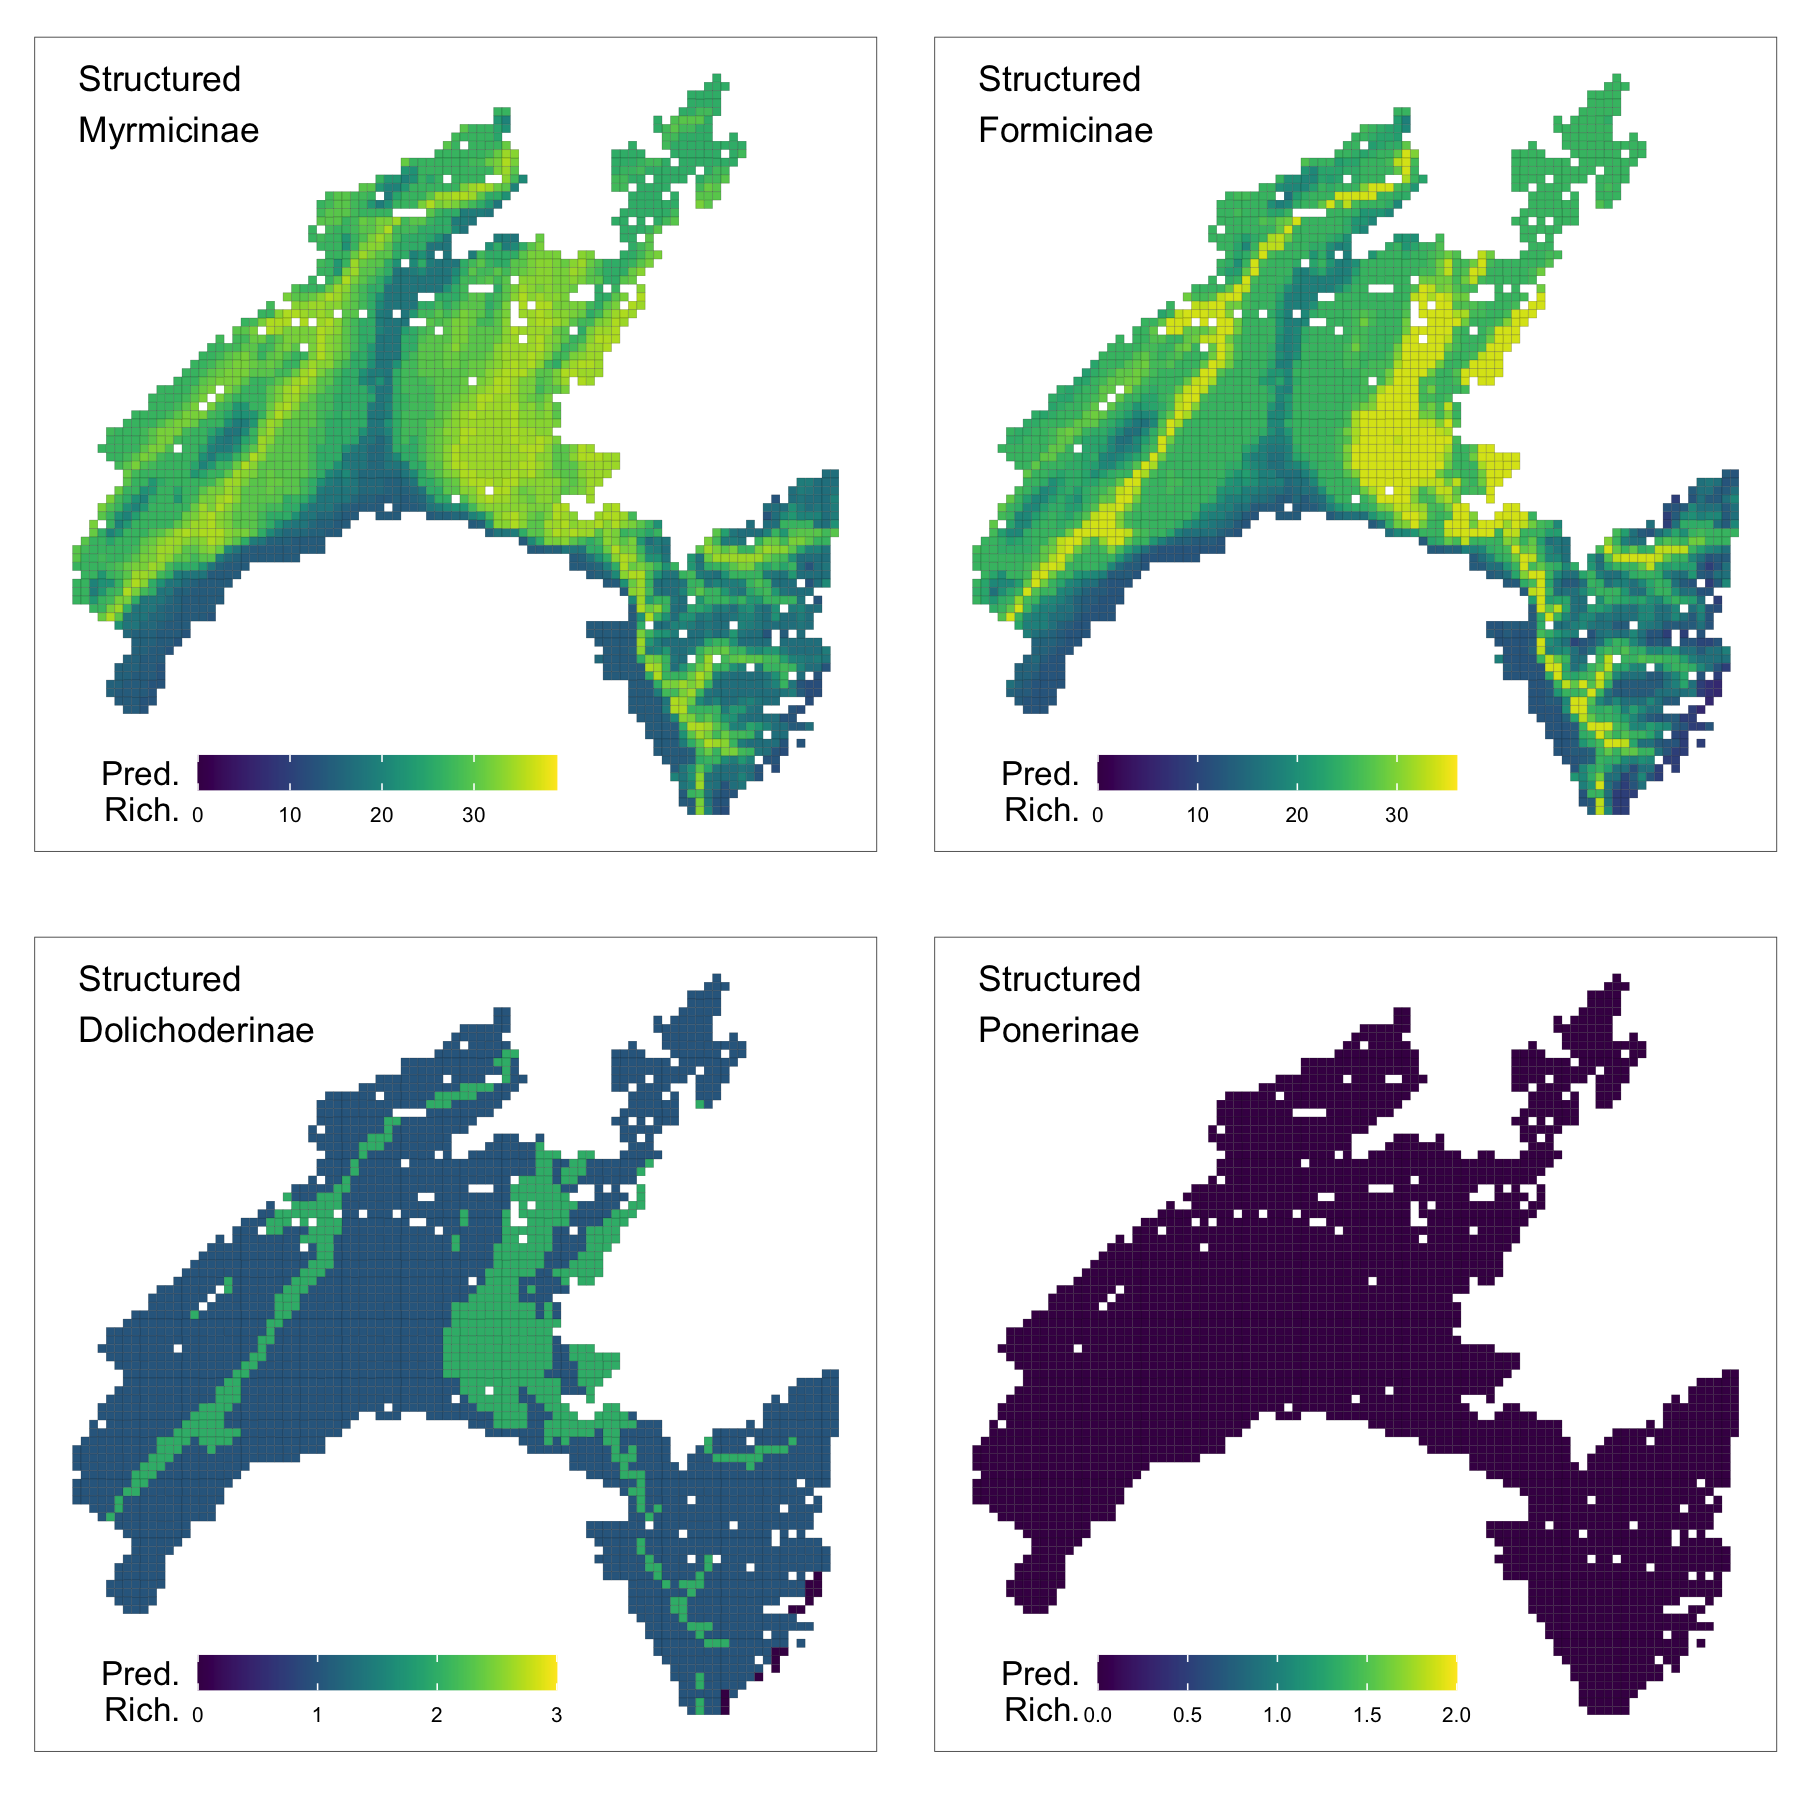
\includegraphics[width=5in]{ms/1_Ecography/1/figs/maps/sf_S_Y.png}
	\caption{\label{fig:sf_map_Structured} Maps of predicted richness in the \emph{Structured} model for subfamilies. Predictions are based on 95\% Highest Posterior Density Intervals for each species. }
\end{figure}

\begin{figure}
	\centering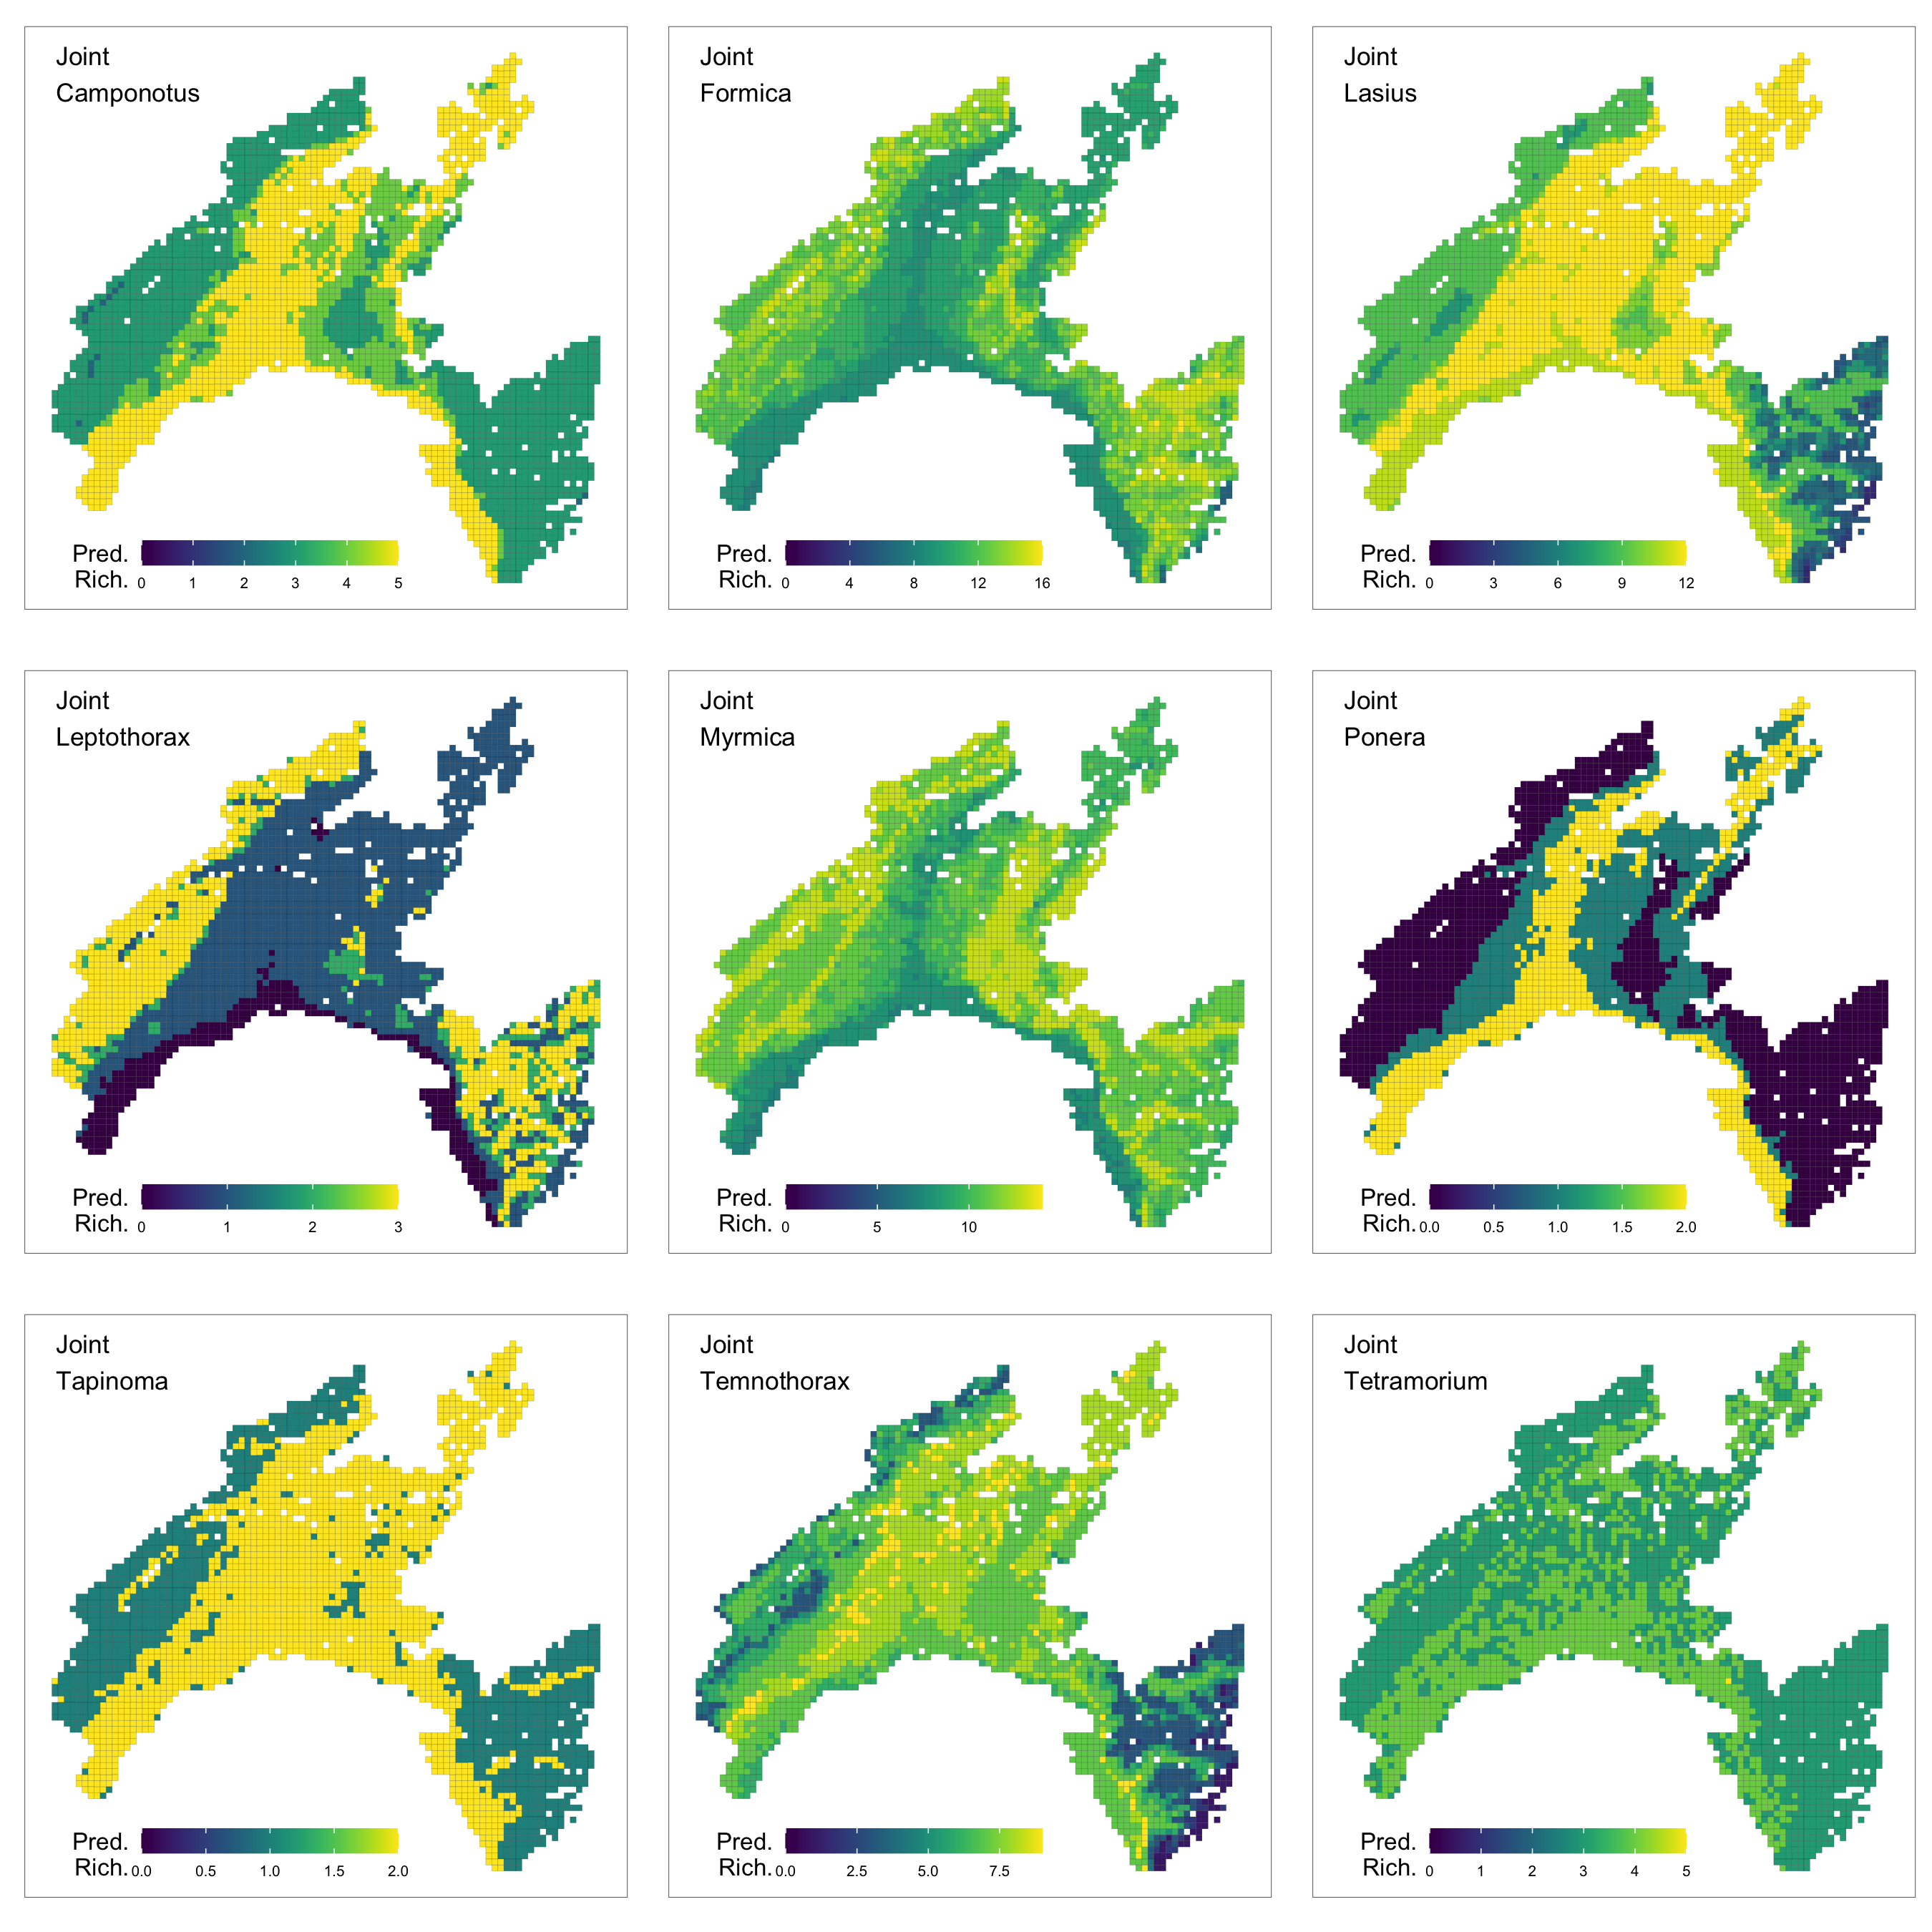
\includegraphics[width=6in]{ms/1_Ecography/1/figs/maps/gen_S_WY.png}
	\caption{\label{fig:gen_map_Joint} Maps of predicted richness in the \emph{Joint} model for genera with at least two species. Predictions are based on 95\% Highest Posterior Density Intervals for each species. }
\end{figure}

\begin{figure}
	\centering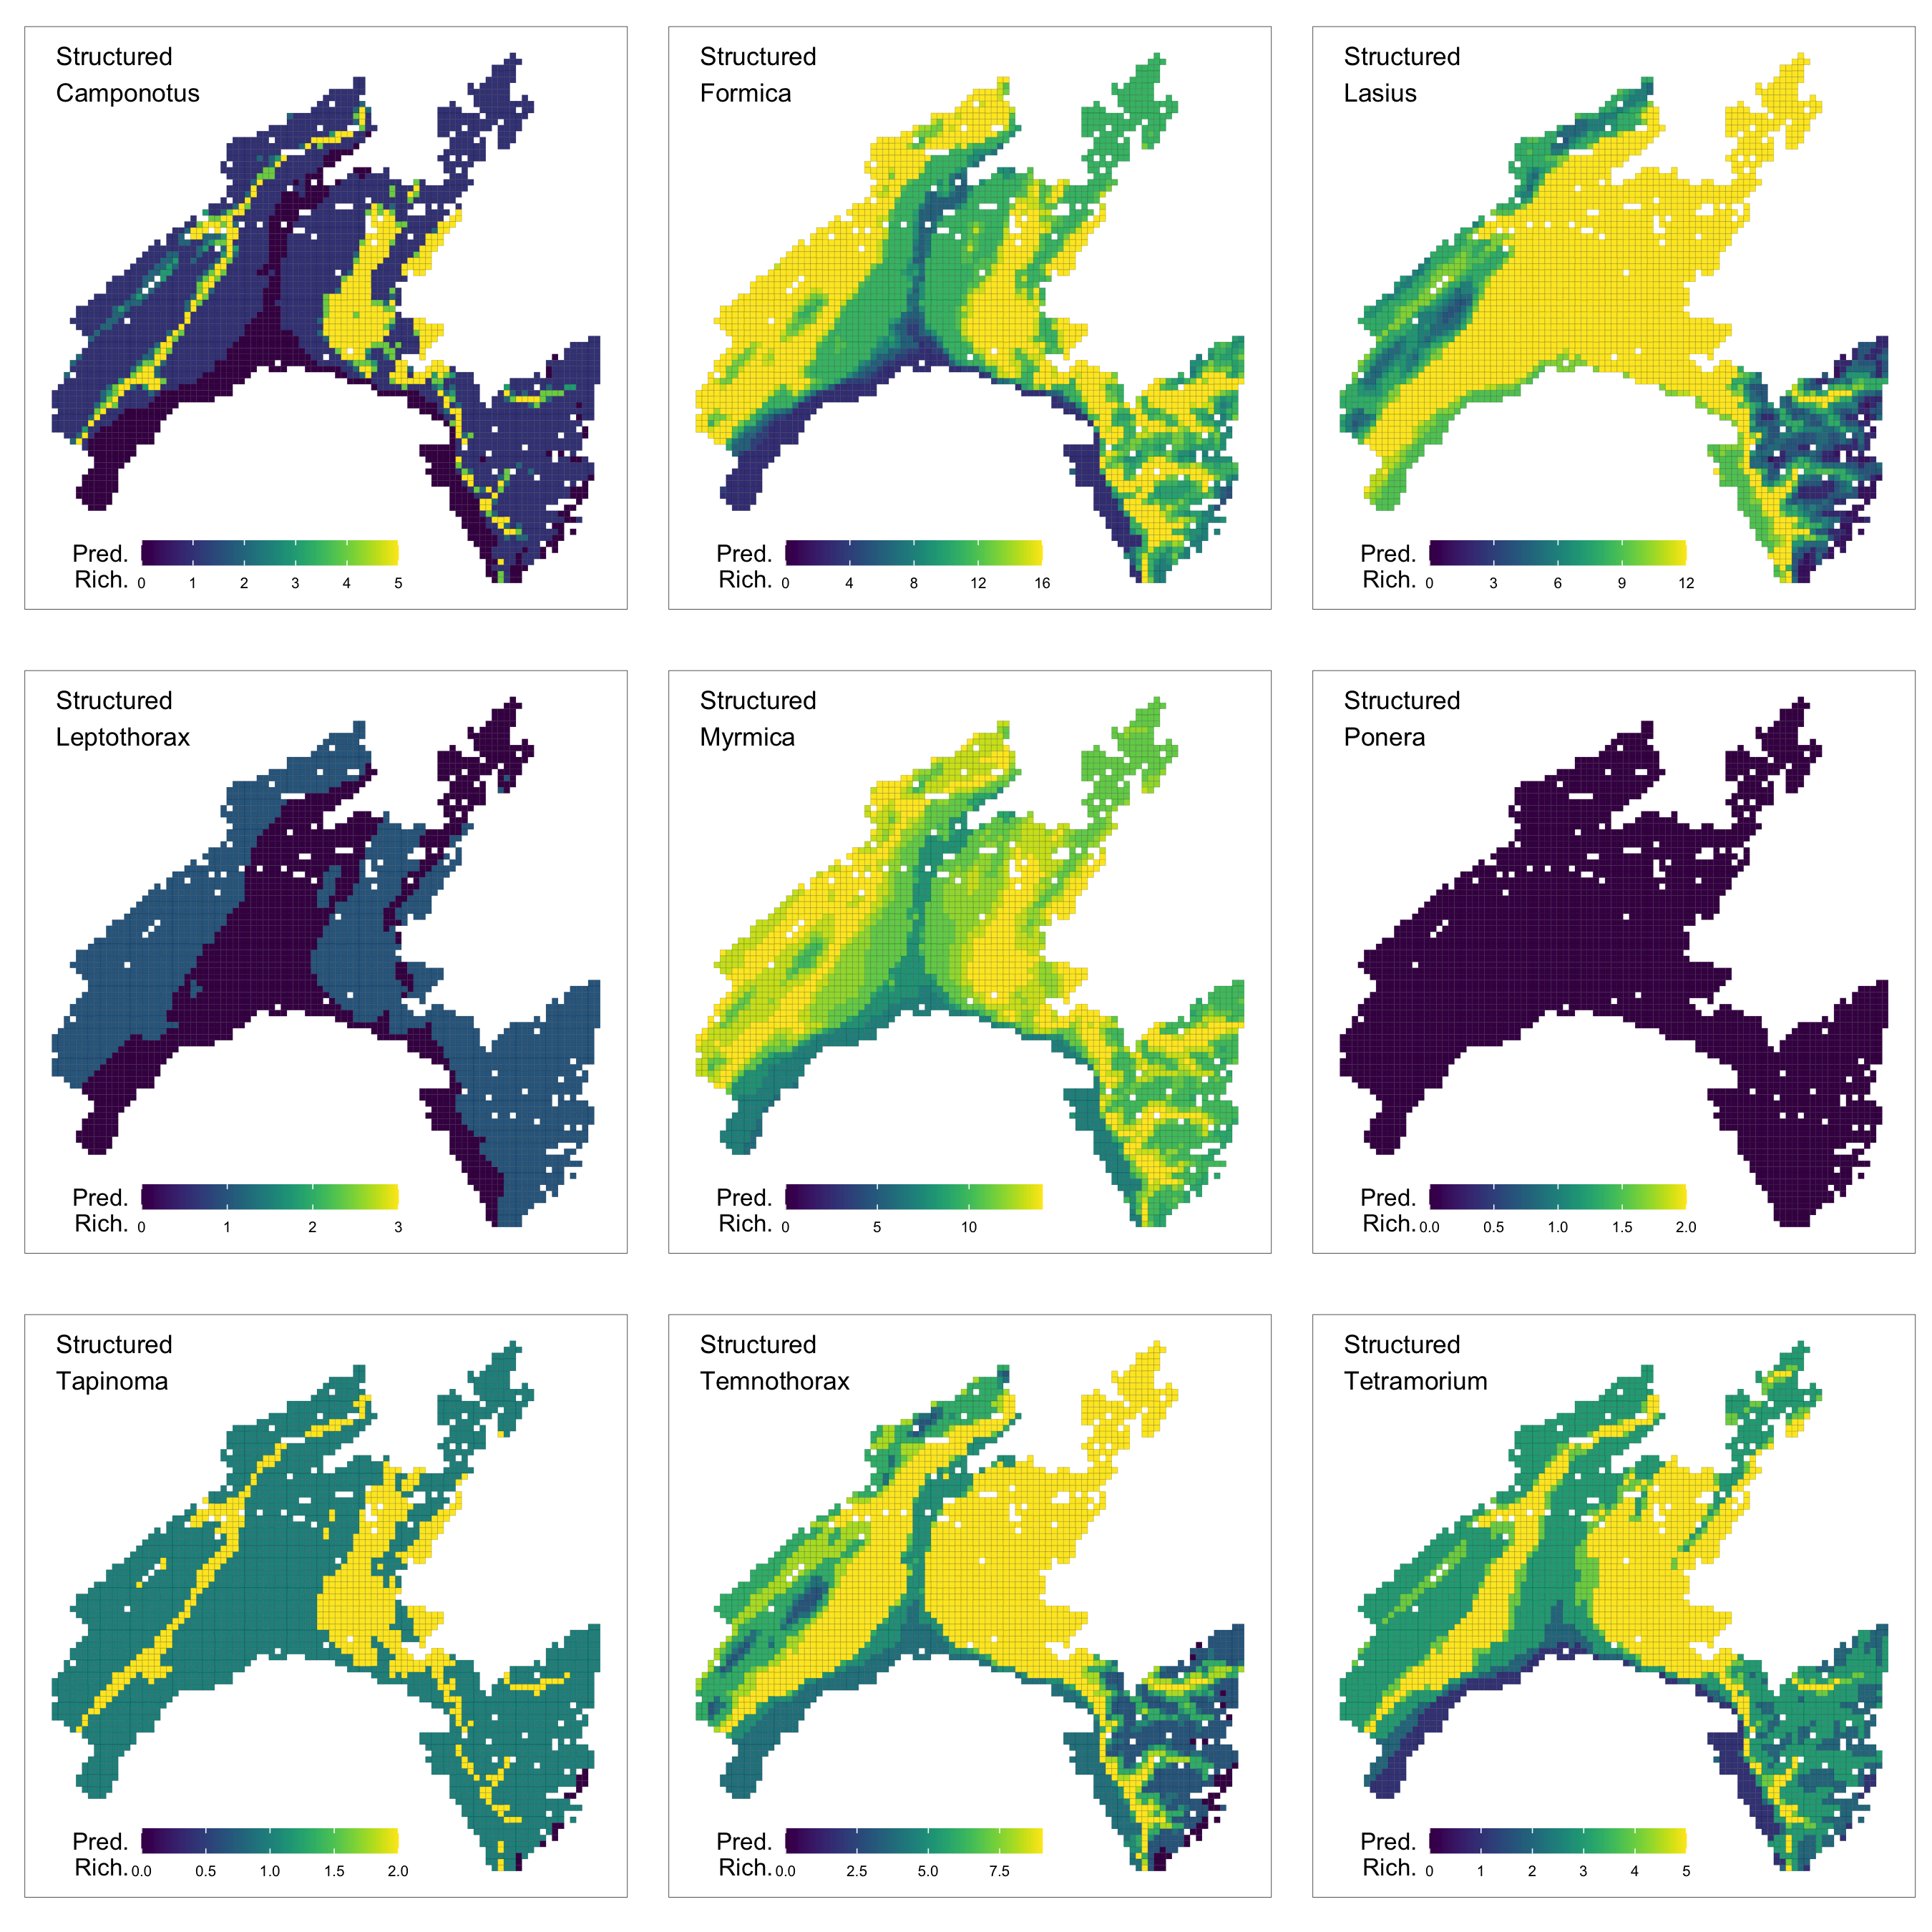
\includegraphics[width=6in]{ms/1_Ecography/1/figs/maps/gen_S_Y.png}
	\caption{\label{fig:gen_map_Structured} Maps of predicted richness in the \emph{Structured} model for genera with at least two species. Predictions are based on 95\% Highest Posterior Density Intervals for each species. }
\end{figure}







\end{document}
